\documentclass[11pt,letterpaper]{article}

\usepackage[utf8]{inputenc}
\usepackage[T1]{fontenc}
\usepackage[margin=1.0in]{geometry}
\usepackage{authblk}
\usepackage{tabularx,booktabs}
\usepackage{multirow}
\usepackage{graphicx}
\graphicspath{{./}}
\usepackage{amsmath,amssymb}
\usepackage{placeins}
\usepackage{microtype}
\usepackage[labelfont=bf]{caption}
\usepackage[hidelinks]{hyperref}
\setlength{\emergencystretch}{3em}  % lets long identifiers (e.g. ChEMBL IDs) break without overfull lines

\renewcommand{\thesection}{\Alph{section}}
\renewcommand{\thetable}{S\arabic{table}}
\renewcommand{\thefigure}{S\arabic{figure}}
\renewcommand{\theequation}{S\arabic{equation}}

\begin{document}

\title{Supplementary Material\\[0.5em]\large Graph-Informed Fusion for Inductive Drug-Target Interaction Prediction and Compound Prioritization in Lung Cancer}

\author[1,2]{Luis H. M. Torres}
\author[3]{Sumaiya Iqbal}
\author[1]{Ashley Mae Conard}
\affil[1]{\small Microsoft Research, Cambridge, MA, USA}
\affil[2]{\small Centre for Informatics and Systems of the University of Coimbra, Department of Informatics Engineering, Univ Coimbra, Coimbra, Portugal}
\affil[3]{\small Broad Institute of MIT and Harvard}


\date{}

\maketitle

\noindent Supplementary material to the main paper: data (Appendix~\ref{app:data}), features, splits, and negatives (Appendix~\ref{app:setting}), architecture (Appendix~\ref{app:architecture}), training procedure and hyperparameters (Appendix~\ref{sec:training}), evaluation protocol and baselines (Appendix~\ref{sec:evaluation}), additional results (Appendix~\ref{sec:results}), attribution controls and extended comparisons (Appendix~\ref{sec:attribution}), and robustness analyses (Appendix~\ref{sec:robustness}). Tables, figures, and equations are numbered with the prefix S. Values are mean $\pm$ standard deviation over 30 training runs (seeds 42-71); unless stated otherwise, paired comparisons between methods use two-sided Wilcoxon signed-rank tests over the 30 runs. Code: \url{https://github.com/ashleyatmsft/gift}.

\section{Data and Knowledge Graph}
\label{app:data}

The dataset was curated for the lung cancer domain and integrates chemical structure, protein target information, bioactivity, and network-level biological relationships into a unified graph representation for DTI learning. The knowledge graph combines compounds, protein targets, compound-protein interactions, protein-protein interactions, and compound-compound relationships. The primary graph was constructed from ChEMBL~35 \cite{zdrazil2024chembl}. A held-out external set of compounds outside the graph, with their activities retrieved from ChEMBL~36, is used only for evaluation (Section~\ref{sec:external_set}). The corresponding scripts are provided in the public code repository.

\paragraph{Compound data collection and clinical-stage filtering}
Compounds were curated from ChEMBL using standardized identifiers, SMILES strings, InChI representations, and molecular properties. Lung cancer-relevant compounds were retained when associated with lung cancer-related targets, indications, or curated bioactivity records involving proteins relevant to lung cancer biology. Compounds were annotated with their development status where available: (i) FDA- or EMA-approved for lung cancer, (ii) under clinical investigation, or (iii) in preclinical development. Including multiple development stages allows the graph to represent both established agents and less characterized candidates. Molecular descriptors and fingerprints were computed with RDKit \cite{landrum_rdkit}.

\paragraph{Target proteins}
Lung cancer-related protein targets were retrieved by cross-referencing ChEMBL, UniProt, and disease-target associations, and retained when associated with lung cancer-related bioactivity, oncogenic signaling, therapeutic relevance, or functional relationships to known lung cancer pathways. The protein set includes major oncogenic drivers, that is, proteins whose activating mutations, gene fusions, or amplifications drive tumor growth, such as EGFR, ALK, ROS1, RET, and MET, as well as proteins involved in signaling, proliferation, survival, DNA damage response, and resistance mechanisms. Each protein was represented by sequence-derived and functional descriptors.

\paragraph{Drug-target interactions (DTIs)}
Compound-protein activity records were retrieved from ChEMBL~35 for 14,453 compound-protein pairs. A pChEMBL value, the standardized negative logarithm of the measured potency, is available for 3,429 of these pairs (23.7\%). The pChEMBL values of a pair are taken from all ChEMBL records of documents released in ChEMBL~35 or earlier, after removing records flagged as potentially erroneous by ChEMBL (data-validity comment), and summarized by their median; 1,494 pairs have more than one value. A median pChEMBL $\geq 5$, which corresponds to a potency of 10~$\mu$M or better, defines an interaction: following this standard activity definition, the 2,865 potent pairs form the compound-protein edges of the graph and provide the positive labels for training and evaluation. The other 11,588 pairs, activity records without a pChEMBL value (11,024 pairs, 76.3\%) or with a median pChEMBL $<5$ (564 pairs), are neither graph edges nor positives, and they are excluded from the evaluation negatives (Section~\ref{sec:evaluation}). The interactions involve 216 of the 1,559 compounds and 793 of the 1,391 proteins; the other compounds are connected to the graph only through compound-compound edges. Median pChEMBL is 6.10 (range 5.00-10.30).

\paragraph{Protein-protein interactions (PPIs)}
Protein-protein interactions among the target proteins were retrieved from STRING \cite{szklarczyk2023string} for \textit{Homo sapiens}, yielding 2,696 interactions that involve 1,113 of the 1,391 proteins. Each edge is weighted by its STRING combined confidence score divided by 1,000, as stored in the graph (range 0.15-0.999, median 0.25); no interaction score threshold above STRING's lowest reported score (0.15) was applied, so low-confidence interactions are included, providing pathway- and network-level context around protein targets.

\paragraph{Compound-compound relationships (CCIs)}
Two types of compound-compound edges were included. \textbf{Similarity edges:} Morgan fingerprints (radius 2, 2,048 bits) \cite{rogers2010extended} were computed with RDKit \cite{landrum_rdkit}, and each compound was linked to at most eight of its most similar compounds with Tanimoto similarity $\geq 0.35$; a compound without such a neighbor was linked to its single most similar compound (59 pairs below 0.35); every compound has at least one structural neighbor (6,927 pairs). \textbf{Therapeutic-class edges:} compounds annotated as therapeutic or in clinical development (maximum phase $>0$) were grouped by their annotated cancer type or indication, and all pairs within a group were connected (2,080 pairs). Both edge types are derived from compound structure and annotations only, not from bioactivity records.

\paragraph{Knowledge graph assembly}
All entities and relations were assembled into a knowledge graph with two node types (compounds and proteins) and three relation types (compound-protein DTIs, protein-protein interactions, and compound-compound edges). The graph was organized in Neo4j \cite{neo4j} for storage and querying, and exported to PyTorch Geometric for training. All edges are represented bidirectionally for message passing.

\paragraph{Final dataset statistics}
The final graph contains 1,559 compounds and 1,391 protein targets (Table~\ref{tab:data_stats}). Compounds are described by 435 features and proteins by 453, and edge attributes are 2-dimensional. Known interactions cover 0.13\% of the 2.17 million possible compound-protein pairs.

\begin{table}
\centering
\caption{Summary statistics of the lung cancer knowledge graph.}
\label{tab:data_stats}
\begin{tabular}{l c}
\toprule
\textbf{Entity / Relation Type} & \textbf{Count} \\
\midrule
Compounds & 1,559 \\
\quad with at least one DTI & 216 \\
Proteins (targets) & 1,391 \\
\quad with at least one DTI & 793 \\
Compound-protein pairs with activity records & 14,453 \\
\quad with a pChEMBL value & 3,429 \\
\quad DTIs (median pChEMBL $\geq 5$) & 2,865 \\
Protein-protein interactions (PPIs) & 2,696 \\
Compound-compound edges (CCIs) & 9,007 \\
\quad Tanimoto similarity & 6,927 \\
\quad therapeutic class & 2,080 \\
Total unique interactions & 14,568 \\
Total directed edges (message passing) & 29,136 \\
Compound / protein feature dimension & 435 / 453 \\
Edge attribute dimension & 2 \\
\midrule
\multicolumn{2}{l}{\textit{External held-out set (ChEMBL~36; not in the graph)}} \\
Compounds & 95 \\
DTIs (median pChEMBL $\geq 5$) at graph proteins & 3,243 \\
Graph proteins with an external DTI & 690 \\
\bottomrule
\end{tabular}
\end{table}



\subsection{External Held-Out Set (ChEMBL~36)}
\label{sec:external_set}
To evaluate the model on compounds that are not part of the knowledge graph, an external held-out set was assembled from ChEMBL~36. It contains 95 small-molecule drugs that are approved for at least one indication (maximum phase 4) and annotated in ChEMBL with a lung cancer indication (MeSH Lung Neoplasms, Non-Small-Cell Lung Carcinoma, or Small Cell Carcinoma): 8 are approved for lung cancer and 87 are under clinical investigation for it (phases 1-3). Examples include the kinase inhibitors crizotinib, erlotinib, brigatinib, and lorlatinib, as well as drugs from other therapeutic areas tested in lung cancer, such as celecoxib, simvastatin, and hydroxychloroquine. None of the 95 compounds is in the ChEMBL~35 graph, and none shares its chemical structure with a graph compound, including stereoisomers and salt forms.

Interactions are defined in the same way as for the graph: for every pair of one of these compounds and one of the 1,391 graph proteins, the pChEMBL values of all ChEMBL~36 records, after removing records flagged by a data-validity comment, are summarized by their median, and a median pChEMBL $\geq 5$ defines an interaction. This yields 3,243 interactions at 690 proteins (median pChEMBL 6.08, range 5.00-10.87), with 4 to 226 active targets per compound (median 17). Every pair with any ChEMBL~36 activity record (22,043 pairs) is recorded as tested, ensuring tested pairs are excluded from the negatives. Compound descriptors are computed with the same definitions as for graph compounds (ChEMBL computed properties and RDKit fingerprints and descriptors) and standardized with the scaler fitted on the ChEMBL~35 graph compounds. The external compounds are added to the graph as nodes without edges, and none of their interactions are used for training, model selection, or feature scaling.

The set is held out with respect to the constructed knowledge graph. Since the graph contains only a curated subset of lung cancer-related compounds, most of these activities were already in ChEMBL before release 36: 96.0\% of the interactions are also interactions when only records from documents released in ChEMBL~35 or earlier are used, and only 129 interactions, on 21 compounds, arise from ChEMBL~36 records. The set therefore measures generalization to compounds outside the training graph. The compounds are also structurally distant from the training compounds (median nearest-neighbor Tanimoto similarity of Morgan fingerprints 0.24, compared with 0.50 for the ChEMBL~35 test compounds of the run with seed 42).

\section{Problem Setting, Features, Splits, and Negatives}
\label{app:setting}
Binary DTI prediction is formulated as link prediction on a heterogeneous graph $\mathcal{G}=(\mathcal{V},\mathcal{E})$ with $|\mathcal{V}_c|=1{,}559$ compound nodes and $|\mathcal{V}_p|=1{,}391$ protein nodes. Each compound $c$ has a descriptor vector $x_c\in\mathbb{R}^{435}$, each protein $p$ a descriptor vector $x_p\in\mathbb{R}^{453}$, and each edge $(i,j)$ an attribute vector $e_{ij}\in\mathbb{R}^{2}$.

\subsection*{Compound Features (435 dimensions)}
All compound features are computed from the chemical structure alone.
\begin{itemize}
    \item \textbf{Molecular descriptors (10):} molecular weight, LogP, H-bond acceptors and donors, rotatable bonds, polar surface area, aromatic rings, heavy atoms, QED, and Lipinski rule-of-five violations (ChEMBL computed properties). The maximum development phase is not used: it is not a structural property, and it correlates with the number of recorded interactions of a compound ($r=0.64$), as approved drugs are tested against more targets.
    \item \textbf{Morgan fingerprint (256):} binary radius-2 circular fingerprint computed with RDKit \cite{rogers2010extended}; every atom environment up to two bonds is hashed into 256 bits.
    \item \textbf{MACCS keys (167):} the complete set of predefined MACCS structural keys \cite{durant2002reoptimization} computed with RDKit; each bit indicates a fixed substructure, such as a functional group, ring type, or atom pair.
    \item \textbf{Saturation and stereochemistry (2):} fraction of sp$^3$ carbons and number of stereocenters, which neither fingerprint encodes.
\end{itemize}

\subsection*{Protein Features (453 dimensions)}
All protein features are computed from the UniProtKB sequence of each target (retrieved by its UniProt accession and available for all 1{,}391 proteins) after removing non-standard residues, or from its annotation; none is derived from interaction records.
\begin{itemize}
    \item \textbf{Annotation features (4):} organism indicators (\textit{H.~sapiens}, \textit{M.~musculus}, \textit{R.~norvegicus}) and a kinase indicator. Features computed from interaction records, such as the number of interacting compounds or the average pChEMBL of a protein, are not used, as they would reveal held-out interactions to every model, including the baselines.
    \item \textbf{Amino-acid composition (20):} relative frequency of each of the 20 standard amino acids.
    \item \textbf{Dipeptide composition (400):} relative frequency of each of the $20\times 20$ ordered pairs of adjacent residues \cite{bhasin2004classification}, which encodes local sequence order.
    \item \textbf{Physicochemical statistics (25):} Kyte-Doolittle hydrophobicity (mean, standard deviation, minimum, maximum, and quartiles), net and mean charge and the numbers of positive and negative residues, aromaticity, fractions of small, medium, and large residues and of polar and non-polar residues, fractions of Cys, Pro, and Gly, and the mean and standard deviation of helix propensity, sheet propensity, and flexibility.
    \item \textbf{Sequence complexity and length (4):} Shannon entropy of the residue distribution, longest single-residue run, length, and log length.
\end{itemize}

Compound and protein features are standardized separately, each with a scaler fitted on the nodes of its own type in the ChEMBL~35 graph; no interaction labels are involved. The two feature sets are placed in disjoint blocks of an 888-dimensional input vector ($[\,$435 compound $|$ 453 protein$\,]$), with zeros in the block of the other type, which is equivalent to type-specific input projections. Compounds of the external set are described with the same descriptor definitions and the same compound scaler.

\subsection*{Edge Features (2 dimensions)}
\begin{itemize}
    \item \textbf{Interaction strength:} median pChEMBL$/12$ for compound-protein edges, STRING confidence for protein-protein edges, and Tanimoto similarity (similarity edges) or a constant 0.5 (therapeutic-class edges) for compound-compound edges.
    \item \textbf{Edge type or evidence:} for compound-protein edges, 1.0 if pChEMBL $> 6$ and 0.5 otherwise; for compound-compound edges, 1.0 for similarity and 0.8 for therapeutic-class edges; for protein-protein edges, this attribute is 0.
\end{itemize}
Only training compound-protein edges, and therefore only training pChEMBL values, are present in the message-passing graph.

\paragraph{Supervision, splits, and graph construction}
Supervision is provided only for compound-protein pairs. In each training run (Section~\ref{sec:evaluation}), the 14,453 pairs with activity records are split at random 70\%/15\%/15\% with the seed of the run, and each part is restricted to its potent pairs. Over the 30 runs, this gives 1,975 to 2,024 training, 402 to 456 validation, and 397 to 455 test interactions (2,020, 402, and 443 in the run with seed 42). Protein-protein and compound-compound edges are not used as labels; they only provide message-passing context.

All validation and test interactions are removed from the graph before any training, in both directions and from every edge list. The message-passing graph, referred to below as the training graph, therefore contains the training interactions and the protein-protein and compound-compound edges, and the same graph is used for training, model selection, and testing. This prevents the model from observing a held-out interaction as an input edge when predicting it \cite{kaufman2012leakage}.

\paragraph{Negative pairs}
Pairs without a potent interaction serve as negatives; they are unlabeled rather than confirmed inactive. Before any training, a fixed random 20\% of all $1{,}559 \times 1{,}391$ compound-protein pairs is reserved for evaluation. Validation and test negatives are drawn only from this reserve and exclude every pair with a ChEMBL~35 activity record, ensuring tested pairs without potent activity are not counted as negatives. Training negatives for every model and every training phase, including the baselines, are drawn from the remaining 80\% and exclude only training interactions. Hence, no model is trained on an evaluation pair. Excluding validation and test interactions from training negatives as well would single them out as the only pairs not labeled negative at any point during training, which a model trained with freshly resampled negatives could learn to recognize. As is standard in link prediction, a few held-out interactions can therefore appear as training negatives; this can only lower the reported performance.

\section{Model Architecture}
\label{app:architecture}
The model has three components: (i) an edge-aware GNN encoder, (ii) a learnable soft-edge module used during representation learning, and (iii) an inductive fusion classifier that combines graph embeddings with descriptor-based encoders (Figure~1 of the main paper; Table~\ref{tab:architecture}). Figure~\ref{fig:detailed} gives a detailed overview of the data, the three components, their training, and the evaluation, with the equations of the following sections.

\begin{figure}[!t]
\centering
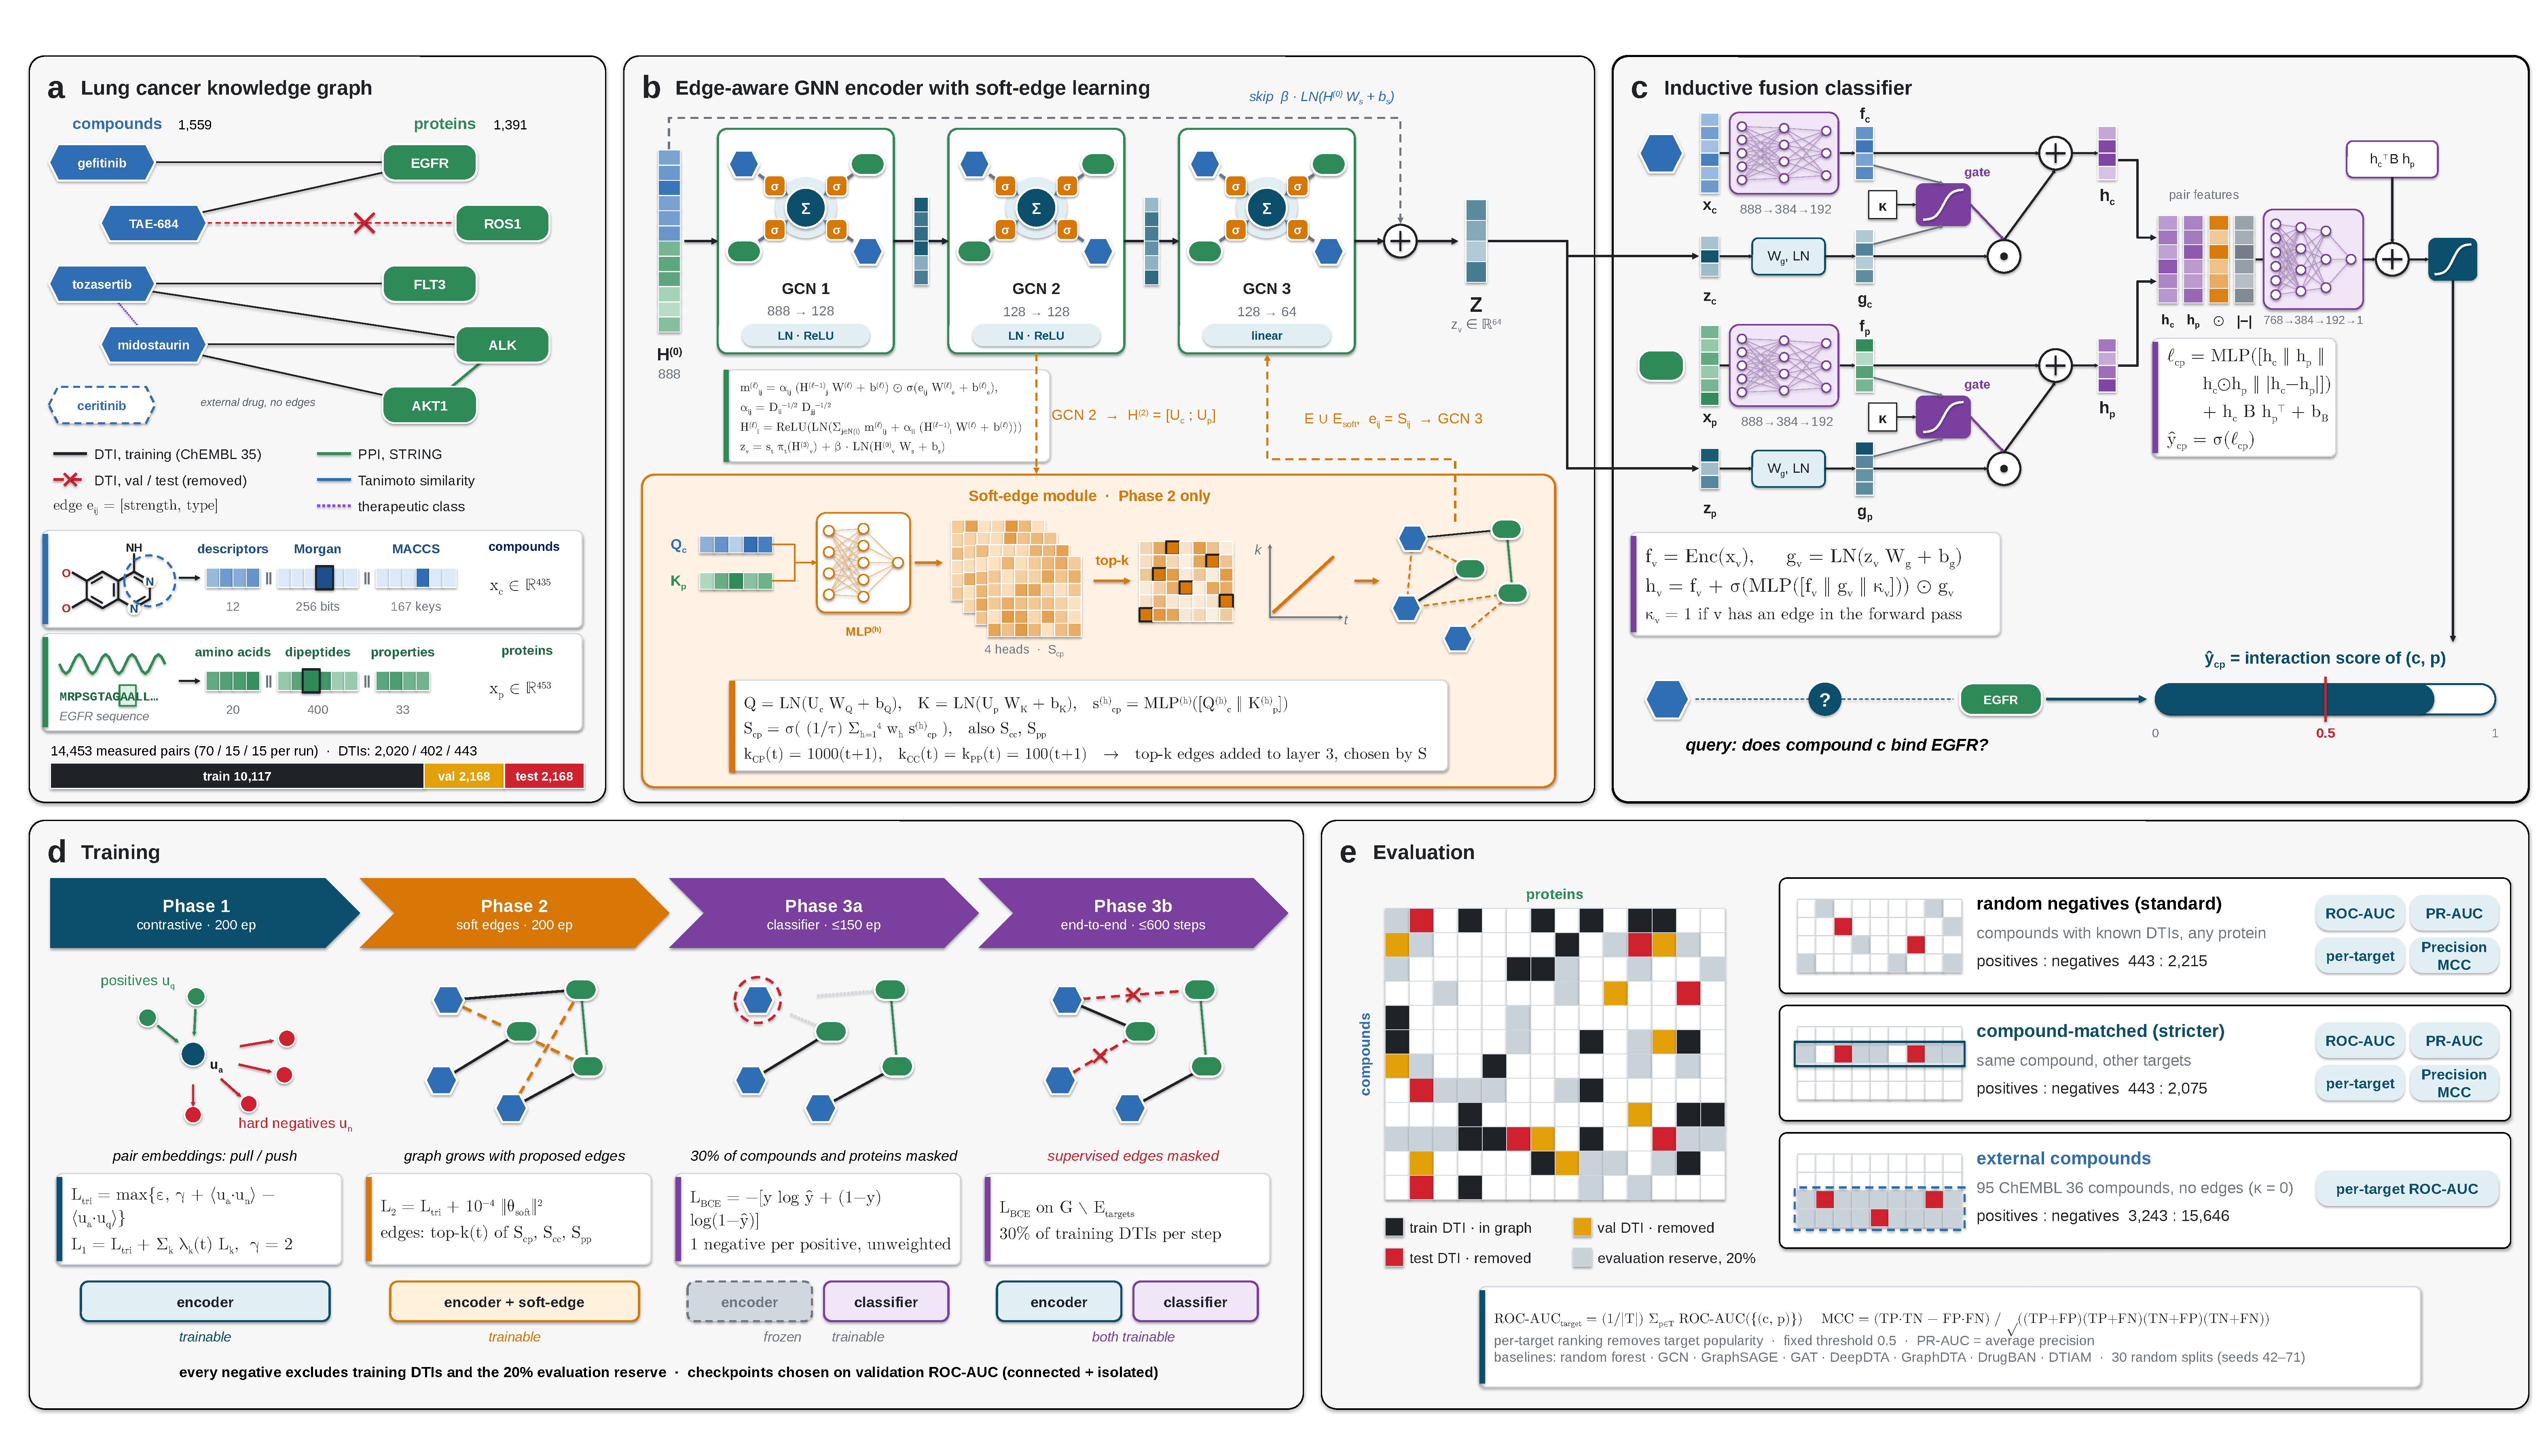
\includegraphics[width=\textwidth]{figs/detailed_overview.pdf}
\caption{Detailed overview of GIFT. (a)~Lung cancer knowledge graph of 1,559 compounds and 1,391 proteins with training DTIs (ChEMBL~35), protein-protein interactions (STRING), and compound-compound edges (Tanimoto similarity and therapeutic class); validation and test DTIs are removed, and the external drugs enter without edges; each edge carries $e_{ij}=[\text{strength},\text{type}]$. Compounds are described by 435 structure-derived features (12 descriptors, 256-bit Morgan fingerprint, 167 MACCS keys) and proteins by 453 sequence-derived features (20 amino-acid and 400 dipeptide frequencies, 33 properties); the 14,453 measured pairs are split 70/15/15 in each run (DTIs 2,020/402/443 for seed 42). (b)~Edge-aware GNN encoder: three edge-gated convolutions ($888\to128\to128\to64$; LayerNorm and ReLU after layers 1 and 2) and a skip connection from the input features give the node embeddings $z_v$ (Section~\ref{sec:encoder}); in Phase~2 only, the soft-edge module scores all candidate pairs from the layer-2 activations with four heads and adds the top-$k(t)$ pairs as weighted edges to layer 3 (Section~\ref{sec:softedge}). (c)~Inductive fusion classifier: descriptor encoders give $f_v$, graph embeddings are projected to $g_v$, a gate with the connectivity flag $\kappa_v$ fuses them into $h_v$, and the pair scorer (MLP and bilinear term) outputs the interaction score $\hat{y}_{cp}$. (d)~Training: Phase~1 contrastive pretraining with hard negatives and consistency terms, Phase~2 soft-edge learning, Phase~3a classifier training on a frozen encoder with 30\% of compounds and proteins masked, and Phase~3b end-to-end fine-tuning with the edges of the supervised interactions removed (Section~\ref{sec:training}). (e)~Evaluation on the three benchmarks (counts for seed 42), with the per-target ROC-AUC and MCC (Section~\ref{sec:evaluation}). Notation is that of the main text (row vectors; every linear map has a bias).}
\label{fig:detailed}
\end{figure}



\subsection{Edge-Aware Graph Convolutions}
\label{sec:encoder}

\paragraph{Inputs and edge sets}
Let $H^{(0)}\in\mathbb{R}^{|\mathcal{V}|\times 888}$ be the block-structured node features. Within the model, every column is additionally rescaled by its mean and standard deviation over all graph nodes, a fixed affine map that is stored with the model and applied unchanged to external compounds. The graph is stored as a set $\mathcal{E}$ of directed edges; every relation appears in both directions with the same attribute vector; thus $e_{ij}=e_{ji}\in\mathbb{R}^2$. During training, each directed edge is kept independently with probability $1-p_{\text{drop}}$, $p_{\text{drop}}=0.15$ (edge dropout \cite{rong2020dropedge}), which gives the edge set $\tilde{\mathcal{E}}$ of the forward pass; at inference, $\tilde{\mathcal{E}}=\mathcal{E}$.

\paragraph{Edge-gated convolution}
Three edge-gated convolution layers map
\[
888 \;\xrightarrow{\;\ell=1\;}\; 128 \;\xrightarrow{\;\ell=2\;}\; 128 \;\xrightarrow{\;\ell=3\;}\; 64.
\]
Node and edge vectors are row vectors. Layer $\ell$ has a node weight matrix $W^{(\ell)}$ with bias $b^{(\ell)}$ and an edge weight matrix $W_e^{(\ell)}\in\mathbb{R}^{2\times d_\ell}$ with bias $b_e^{(\ell)}$. With the in-neighborhood $\mathcal{N}(i)=\{j:(j,i)\in\tilde{\mathcal{E}}\}$ and the degree $D_{ii}=1+|\mathcal{N}(i)|$, which counts the self-loop, and the symmetric normalization $\alpha_{ij} = D_{ii}^{-1/2} D_{jj}^{-1/2}$, the layer computes
\begin{equation}
\tilde{H}^{(\ell)}_i = \alpha_{ii}\big(H^{(\ell-1)}_i W^{(\ell)}+b^{(\ell)}\big) + \sum_{j\in\mathcal{N}(i)} \alpha_{ij}\big(H^{(\ell-1)}_j W^{(\ell)}+b^{(\ell)}\big)\odot\sigma\!\big(e_{ij} W_e^{(\ell)}+b_e^{(\ell)}\big),
\label{eq:conv}
\end{equation}
followed by $H^{(\ell)}=\mathrm{ReLU}\big(\mathrm{LayerNorm}(\tilde{H}^{(\ell)})\big)$ for $\ell=1,2$ and $H^{(3)}=\tilde{H}^{(3)}$. The gate $\sigma(e_{ij}W_e^{(\ell)}+b_e^{(\ell)})\in(0,1)^{d_\ell}$ rescales each channel of a neighbor's message according to the edge attributes; the self-loop term is not gated. Since the relation types and the two compound-protein evidence levels differ in their attribute values, the gate acts as a relation- and evidence-dependent channel weighting with a single set of node weights, instead of one weight matrix per relation as in relational GCNs \cite{schlichtkrull2018modeling}.

\paragraph{Isolated nodes}
For a node $v$ without edges, $\mathcal{N}(v)=\emptyset$ and $D_{vv}=1$; hence $\tilde{H}^{(\ell)}_v=H^{(\ell-1)}_v W^{(\ell)}+b^{(\ell)}$ in every layer, and its embedding is a deterministic function of its own descriptors. This is the situation of external compounds at inference and of the compounds that are isolated during training (Sections~\ref{sec:training} and~\ref{sec:evaluation}).

\paragraph{Node embeddings}
The node embedding $z_v\in\mathbb{R}^{64}$ combines the layer-3 output with a skip connection from the input features,
\[
z_v = s_{t(v)}\,\pi_{t(v)}\big(H^{(3)}_v\big) + \beta\,\mathrm{LayerNorm}\big(H^{(0)}_v W_s + b_s\big),
\]
where $t(v)$ is the node type, $\pi_c$ and $\pi_p$ are separate projection heads for compounds and proteins ($\mathrm{Linear}(64\to128)\to\mathrm{ReLU}\to\mathrm{Dropout}(0.3)\to\mathrm{Linear}(128\to64)\to\mathrm{LayerNorm}$), $s_c=1$, $s_p$ is a learnable protein scale initialized to 2, and $\beta$ is a learnable weight initialized to $0.5$. The embeddings $z_v$ are used by the contrastive objective and by the fusion classifier.

\subsection{Soft-Edge Learning Module}
\label{sec:softedge}
The soft-edge module learns which compound-protein, compound-compound, and protein-protein pairs should be connected to improve the encoder's representations, and adds them to the graph as weighted edges during Phase~2. Unlike most graph structure learning methods (main paper, Section~1), which refine a homogeneous graph for node classification, it proposes edges of three relation types with separate scorers, receives no direct supervision from interaction labels but is trained only through the contrastive objective on the training interactions, and is not used at inference. It operates on the layer-2 activations $U=H^{(2)}$, with compound rows $U_c\in\mathbb{R}^{|\mathcal{V}_c|\times 128}$ and protein rows $U_p\in\mathbb{R}^{|\mathcal{V}_p|\times 128}$.

\paragraph{Candidate pairs}
The candidates are all compound-protein pairs, $\Pi_{\text{CP}}=\mathcal{V}_c\times\mathcal{V}_p$ (2.17 million), and all unordered pairs of distinct nodes of the same type, $\Pi_{\text{CC}}=\{(i,j)\in\mathcal{V}_c^2: i<j\}$ and $\Pi_{\text{PP}}=\{(i,j)\in\mathcal{V}_p^2: i<j\}$, in node index order. Candidates are not filtered against the observed edges and do not depend on any label.

\paragraph{Compound-protein scores}
Queries and keys are $Q=\mathrm{LN}(U_c W_Q+b_Q)$ and $K=\mathrm{LN}(U_p W_K+b_K)$, where $W_Q,W_K\in\mathbb{R}^{128\times128}$ and $\mathrm{LN}$ is layer normalization without learnable parameters. Both are split into $H=4$ heads of dimension $d_h=32$, $Q^{(h)}_c,K^{(h)}_p\in\mathbb{R}^{32}$. Each head scores a pair with its own MLP on the concatenated query and key, and the heads are combined with learned weights and a learned temperature:
\begin{equation}
s^{(h)}_{cp} = \mathrm{MLP}^{(h)}\big([Q_c^{(h)}\,\|\,K_p^{(h)}]\big),
\qquad
S_{cp} = \sigma\!\Big(\frac{1}{\tau}\sum_{h=1}^{H} w_h\, s^{(h)}_{cp}\Big),
\qquad w=\mathrm{softmax}(\omega),
\label{eq:softedge}
\end{equation}
where $\mathrm{MLP}^{(h)}$ is $\mathrm{Linear}(64\to32)\to\mathrm{LayerNorm}\to\mathrm{GELU}\to\mathrm{Dropout}(0.1)\to\mathrm{Linear}(32\to16)\to\mathrm{GELU}\to\mathrm{Linear}(16\to1)$, $\omega\in\mathbb{R}^{4}$ is initialized uniformly, and $\tau$ is initialized to $0.5$. Unlike dot-product attention \cite{vaswani2017attention}, each head is a nonlinear function of the query-key pair, and the scores are not normalized over the candidates of a node; every pair therefore receives an independent score $S_{cp}\in(0,1)$.

\paragraph{Homogeneous scores}
For $(i,j)\in\Pi_{\text{CC}}$, and analogously for $\Pi_{\text{PP}}$ with separate parameters,
\[
S_{ij} = \sigma\!\Big(\sum_{h=1}^{H} w'_h\, \mathrm{MLP}'^{(h)}\big([Q'^{(h)}_i\,\|\,K'^{(h)}_j]\big)\Big),
\qquad Q'=UW'_Q+b'_Q,\quad K'=UW'_K+b'_K,
\]
with $W'_Q,W'_K\in\mathbb{R}^{128\times128}$ and no normalization, two-layer heads $\mathrm{Linear}(64\to32)\to\mathrm{LayerNorm}\to\mathrm{GELU}\to\mathrm{Dropout}(0.1)\to\mathrm{Linear}(32\to1)$, softmax-normalized head weights $w'$, and no temperature. The query-key form is not symmetric; each unordered pair is scored once, with the lower-index node as the query.

\paragraph{Progressive top-$k$ selection}
At epoch $t\in\{0,\dots,199\}$ of Phase~2, the module keeps the highest-scoring candidates of each type $r\in\{\text{CP},\text{CC},\text{PP}\}$,
\[
\mathcal{E}^{(t)}_r = \operatorname{TopK}_{k_r(t)}\big\{S_{ij} : (i,j)\in\Pi_r\big\},
\qquad k_{\text{CP}}(t)=1000\,(t+1),\qquad k_{\text{CC}}(t)=k_{\text{PP}}(t)=100\,(t+1).
\]
The last epoch therefore proposes 200,000 compound-protein edges (9.2\% of the candidates) and 20,000 edges of each homogeneous type. The linear schedule first adds a small number of the highest-scoring pairs and exposes the encoder to progressively larger neighborhoods as training proceeds.

\paragraph{Augmented propagation}
Each selected pair is added in both directions with the attribute vector $e_{ij}=e_{ji}=(S_{ij},S_{ij})$, which gives the proposed edge set $\mathcal{E}^{(t)}_{\text{soft}}=\bigcup_r\{(i,j),(j,i):(i,j)\in\mathcal{E}^{(t)}_r\}$. Layers 1 and 2 run on the observed graph $\tilde{\mathcal{E}}$, and layer 3 is computed with Eq.~\eqref{eq:conv} on $\tilde{\mathcal{E}}\cup\mathcal{E}^{(t)}_{\text{soft}}$, including in the degrees $D_{ii}$; a proposed pair that is already an observed edge is added a second time. For a proposed edge, the message gate of Eq.~\eqref{eq:conv} becomes $\sigma\big(S_{ij}\,(w^{(3)}_{e,1}+w^{(3)}_{e,2})+b^{(3)}_e\big)$, where $w^{(3)}_{e,1}$ and $w^{(3)}_{e,2}$ are the two rows of the layer-3 edge weight matrix and $b^{(3)}_e$ its bias; each channel is therefore a monotone function of the score, and $S_{ij}$ controls how strongly the proposed neighbor contributes to the final embedding.

\paragraph{Gradient path and supervision}
The top-$k$ selection is piecewise constant in the scores and passes no gradient. Gradients reach the module only through the scores of the selected pairs, via their edge gates in layer~3: $\partial\mathcal{L}/\partial S_{ij}\neq 0$ only for $(i,j)\in\mathcal{E}^{(t)}_r$. From there they propagate into the scoring MLPs, the query and key maps, and, through $U$, into layers 1 and 2 of the encoder. The module is trained only by the Phase~2 contrastive objective: it increases the scores of proposed edges whose messages reduce the triplet loss and decreases the others, which can move them out of the top-$k$ set in later epochs. No interaction label is used as a target for the scores; training interactions influence them only indirectly, through the triplet loss, and validation and test interactions have no influence on them. The module scores all compound-protein pairs, including held-out pairs; a held-out interaction can be proposed only if the learned scores rank it highly.

\paragraph{Use at inference}
The soft-edge module shapes the encoder during representation learning (Phase~2). At inference, embeddings are computed on the observed training graph without the proposed edges.

\subsection{Inductive Fusion Classifier}
Graph embeddings are informative for well-connected nodes but uninformative for compounds without known interactions, such as compounds outside the training graph. The classifier therefore combines two views of each node.

\paragraph{Descriptor encoders}
Separate compound and protein encoders $T_c$ and $T_p$ map the rescaled block inputs $x_v$ (the rows of $H^{(0)}$) to $f_v=T_{t(v)}(x_v)\in\mathbb{R}^{192}$:
\[
\begin{aligned}
T_t:\ &\mathrm{Dropout}(0.1)\to\mathrm{Linear}(888\to 384)\to\mathrm{LayerNorm}\to\mathrm{GELU}\\
&\quad\to\mathrm{Dropout}(0.25)\to\mathrm{Linear}(384\to 192)\to\mathrm{LayerNorm}.
\end{aligned}
\]
These encoders are inductive and apply to any compound or protein, whether or not it has edges in the graph.

\paragraph{Gated fusion}
Graph embeddings $z_v\in\mathbb{R}^{64}$ are projected to $g_v=\mathrm{LayerNorm}(z_v W_g + b_g)\in\mathbb{R}^{192}$. For each node, a gate determines the amount of graph evidence added to the descriptor representation $f_v$:
\[
h_v = f_v + \sigma\!\big(\mathrm{MLP}([f_v\,\|\,g_v\,\|\,\kappa_v])\big)\odot g_v,
\]
where the MLP maps $385\to192\to192$ with a GELU, such that the sigmoid gate acts on each dimension separately, and $\kappa_v\in\{0,1\}$ indicates whether the node has at least one edge of any type in the graph of the current forward pass, before edge dropout; masked compounds and proteins (Section~\ref{sec:training}) and external compounds therefore have $\kappa_v=0$. For such nodes, $g_v$ is computed from the isolated-node embedding, which depends only on $x_v$ (Section~\ref{sec:encoder}), and the gate can learn to down-weight it. Compounds and proteins have separate graph projections and gates. The gate receives only this binary flag rather than node degree, which prevents the classifier from using the number of known interactions as a shortcut.

\paragraph{Pair scorer}
For a pair $(c,p)$, the interaction logit is
\[
\ell_{cp} = \mathrm{MLP}\big([h_c\,\|\,h_p\,\|\,h_c\odot h_p\,\|\,|h_c-h_p|]\big) + h_c B\, h_p^{\top} + b_B,
\qquad \hat{y}_{cp}=\sigma(\ell_{cp}),
\]
with an MLP that applies LayerNorm to the 768-dimensional input followed by $\mathrm{Linear}(768\to384)\to\mathrm{GELU}\to\mathrm{Dropout}(0.25)\to\mathrm{Linear}(384\to192)\to\mathrm{GELU}\to\mathrm{Linear}(192\to1)$, and a learned bilinear form $B\in\mathbb{R}^{192\times192}$ with bias $b_B$.

\begin{table}[!h]
\centering
\caption{Model architecture and training hyperparameters.}
\label{tab:architecture}
\begin{tabularx}{\textwidth}{l X}
\toprule
\textbf{Component / Hyperparameter} & \textbf{Value} \\
\midrule
Input feature dimension & 888 (435 compound + 453 protein block) \\
GNN dimensions & $888\to128\to128\to64$ (edge-gated GCN) \\
Embedding output & type-specific projection heads $64\to128\to64$ + skip $\mathrm{LayerNorm}(H^{(0)}W_s+b_s)$ \\
Normalization (GNN) & LayerNorm \\
Training edge dropout & 0.15 \\
Soft-edge module & 4 heads, $d_h=32$; top-$k$ $1000(t+1)$ C-P, $100(t+1)$ C-C and P-P \\
Soft-edge $L_2$ penalty & $10^{-4}$ (compound-protein scorer) \\
Descriptor encoders & $888\to384\to192$ \\
Fusion / pair scorer & gated fusion; MLP $768\to384\to192\to1$ + bilinear \\
\midrule
Phases 1-2 & Adam, lr $10^{-4}$, 200 + 200 epochs \\
Triplet margin / negatives per positive & 2.0 / 10 (70\% hard, 30\% random) \\
Phase 3a (head) & AdamW, lr $10^{-3}$, wd $10^{-4}$, cosine, batch 512, $\leq$150 epochs \\
Phase 3b (end-to-end) & AdamW, lr $2\!\times\!10^{-5}$ (GNN) / $2\!\times\!10^{-4}$ (head), $\leq$600 steps \\
Classification negatives & 1 per positive, resampled; unweighted BCE \\
Node masking (Phase 3) & 0.30 of compounds and 0.30 of proteins per epoch/step \\
Decision threshold & 0.5 (fixed) \\
Total parameters & 1,904,414 \\
\quad fusion classifier / soft-edge module & 1,488,770 / 185,113 \\
\bottomrule
\end{tabularx}
\end{table}

\section{Training Procedure}
\label{sec:training}

\paragraph{Overview}
Training proceeds in three phases. Phases~1 and~2 learn node embeddings with a contrastive objective and do not involve the classifier. Phase~3 trains the fusion classifier, first on a frozen encoder (Phase~3a) and then jointly with the encoder (Phase~3b). Every phase operates on the training graph, in which the training interactions are the only compound-protein edges, and every phase draws its training negatives under the rule described above: negatives exclude both training interactions and pairs of the evaluation reserve. The graph is small enough to be processed in full; each forward pass computes embeddings for all 2,950 nodes and only the supervised pairs are sub-sampled. Gradients are clipped to a norm of 1.0 in every phase.

In Phase~1 (contrastive pretraining), the encoder is trained with a triplet loss on the training interactions and four consistency terms, on the observed graph with edge dropout of 0.15 and an extra forward pass in which up to 20\% of the compounds are isolated, that is, have all their edges removed; the checkpoint with the lowest validation triplet loss is kept (200 epochs, early stopping with patience 80). In Phase~2 (soft-edge learning), the encoder and the soft-edge module are trained with the triplet loss and an $L_2$ penalty on the compound-protein scorer, on the observed graph extended with the proposed edges (progressive top-$k$) and with edge dropout of 0.15; the checkpoint with the lowest validation triplet loss over 200 epochs is kept. In Phase~3a (classifier), only the fusion classifier is trained, with the binary cross-entropy and one negative per positive, while 30\% of the compounds and 30\% of the proteins are masked (all their edges removed) and resampled every epoch; it runs for at most 150 epochs with patience 20. In Phase~3b (end-to-end), the encoder and the fusion classifier are trained jointly with the binary cross-entropy on 30\% of the training interactions per step, whose edges are removed from the graph, with 30\% of the compounds and 30\% of the proteins masked and edge dropout of 0.15; it runs for at most 600 steps and is evaluated every 10 steps, with patience 12 evaluations. Both Phase~3 stages select checkpoints on the validation area under the receiver operating characteristic curve (ROC-AUC) over two views of the graph, the standard selection criterion in DTI prediction. Validation interactions are absent from the graph in every phase.

\subsection{Phase 1: Contrastive Pretraining}

\paragraph{Pair embeddings}
For a compound $c$ and a protein $p$ with encoder outputs $z_c,z_p\in\mathbb{R}^{64}$, the pair embedding is the normalized concatenation of the normalized node embeddings,
\[
u_{cp} = \frac{[\hat{z}_c \,\|\, \hat{z}_p]}{\big\|[\hat{z}_c \,\|\, \hat{z}_p]\big\|},
\qquad \hat{z} = z/\|z\|,
\]
such that the similarity of two pairs, $\langle u_a,u_b\rangle$, is a cosine similarity in $[-1,1]$.

\paragraph{Eligible negatives and hard-negative mining}
Let $\mathcal{E}^{+}$ denote the training interactions and $\mathcal{R}$ the evaluation reserve. A pair is an eligible negative if it belongs to
\[
\Omega = (\mathcal{V}_c\times\mathcal{V}_p)\setminus(\mathcal{E}^{+}\cup\mathcal{R}).
\]
In each epoch, a batch $\mathcal{B}$ of 64 anchors is drawn without replacement from $\mathcal{E}^{+}$. For each anchor $a=(c,p)$, a candidate set is formed from three sources,
\[
\mathcal{C}_a = \mathcal{C}_a^{\text{comp}}\cup\mathcal{C}_a^{\text{prot}}\cup\mathcal{C}_a^{\text{rand}},
\]
where $\mathcal{C}_a^{\text{comp}}$ contains 50 pairs $(c,p')\in\Omega$ drawn uniformly without replacement among the eligible pairs of compound $c$, $\mathcal{C}_a^{\text{prot}}$ contains 50 pairs $(c',p)\in\Omega$ drawn in the same way for protein $p$, and $\mathcal{C}_a^{\text{rand}}$ contains the eligible pairs among 30 uniformly random compound-protein pairs. The candidates are ranked by their current similarity to the anchor, $\langle u_a,u_n\rangle$, computed without gradient, and the negative set $\mathcal{N}_a$ consists of the 7 most similar candidates and 3 candidates drawn uniformly from the rest (70\% hard, 30\% random); thus $|\mathcal{N}_a|=10$. Negatives are mined online from the embeddings of the current epoch \cite{schroff2015facenet, hermans2017defense}. Since 100 of the at most 130 candidates share the compound or the protein of the anchor, the encoder must distinguish a compound's targets from its non-targets, and a protein's ligands from its non-ligands, rather than recognize frequently tested compounds or proteins.

\paragraph{Positive reference}
For each anchor, 20 other training interactions are drawn uniformly; pooled over the batch, they form a set $\mathcal{P}$ of $64\times20=1{,}280$ pairs that is shared by all anchors of the batch.

\paragraph{Triplet loss}
The contrastive loss is
\begin{equation}
\mathcal{L}_{\text{tri}} = \frac{1}{|\mathcal{B}|}\sum_{a\in\mathcal{B}} \max\!\Big\{\epsilon,\ \gamma + \frac{1}{|\mathcal{N}_a|}\sum_{n\in\mathcal{N}_a} \langle u_a,u_n\rangle - \frac{1}{|\mathcal{P}|}\sum_{q\in\mathcal{P}} \langle u_a,u_q\rangle \Big\},
\label{eq:triplet}
\end{equation}
with margin $\gamma=2$ and floor $\epsilon=10^{-4}$. Since every similarity lies in $[-1,1]$, the term inside the hinge is at least $\gamma-2=0$; the hinge remains active for every anchor and, up to the floor $\epsilon$,
\[
\mathcal{L}_{\text{tri}} = \gamma + \frac{1}{|\mathcal{B}|}\sum_{a\in\mathcal{B}}\Big(\overline{\mathrm{sim}}(a,\mathcal{N}_a) - \overline{\mathrm{sim}}(a,\mathcal{P})\Big),
\]
where $\overline{\mathrm{sim}}$ denotes the mean cosine similarity of the anchor to a set. Every anchor therefore contributes a gradient in every epoch: the loss moves each interacting pair toward the other interacting pairs and away from its hardest non-interacting pairs. Unlike a standard triplet loss, in which the positive shares the identity of the anchor \cite{schroff2015facenet}, the positive term compares the anchor with a pool of other interactions; interacting pairs are thereby gathered into a common region of the pair space.

\paragraph{Consistency regularizers}
Two additional forward passes are computed in each epoch, with the encoder in training mode, and gradients flow through all passes. These terms use the unnormalized concatenation $v_{cp}=[z_c\,\|\,z_p]$. The second pass runs on the same graph as the main pass and differs only through independently resampled edge dropout and projection-head dropout; its embeddings $z'$ are aligned with those of the main pass by two view terms,
\[
\mathcal{L}_{\text{view}} = 1 - \frac{1}{2}\Big[\frac{1}{|\mathcal{V}_c|}\sum_{c}\cos(z_c,z'_c) + \frac{1}{|\mathcal{V}_p|}\sum_{p}\cos(z_p,z'_p)\Big],
\qquad
\mathcal{L}_{\text{view-pair}} = 1 - \frac{1}{|\mathcal{S}|}\sum_{(c,p)\in\mathcal{S}}\cos(v_{cp},v'_{cp}),
\]
where $\mathcal{S}$ contains all training interactions (at most 2,048 are sampled). In the third pass, a random set $I_t$ of $\mathrm{round}(\rho_t|\mathcal{V}_c|)$ compounds, resampled every epoch, is isolated by removing all their edges in both directions, and edge dropout is applied to the remaining edges. Two isolation terms align the embeddings of the isolated compounds, and of their training interactions, with their counterparts from the main pass:
\[
\mathcal{L}_{\text{iso}} = 1 - \frac{1}{|I_t|}\sum_{c\in I_t}\cos\big(z_c, z_c^{\text{iso}}\big),
\qquad
\mathcal{L}_{\text{iso-pair}} = 1 - \frac{1}{|\mathcal{S}_I|}\sum_{(c,p)\in\mathcal{S}_I}\cos\big(v_{cp}, v_{cp}^{\text{iso}}\big),
\]
where $\mathcal{S}_I$ contains up to 2,048 training interactions whose compound is in $I_t$. Since an isolated compound's embedding depends only on its descriptors (Section~\ref{sec:encoder}), $\mathcal{L}_{\text{iso}}$ pulls the graph-based embedding of each compound toward a function of its descriptors alone, which is the representation that compounds outside the graph receive. The Phase~1 objective is
\begin{equation}
\mathcal{L}_1 = \mathcal{L}_{\text{tri}} + \lambda_{\text{iso}}(t)\,\mathcal{L}_{\text{iso}} + \lambda_{\text{iso-pair}}(t)\,\mathcal{L}_{\text{iso-pair}} + \lambda_{\text{view}}(t)\,\mathcal{L}_{\text{view}} + \lambda_{\text{view-pair}}(t)\,\mathcal{L}_{\text{view-pair}},
\end{equation}
where every weight increases linearly from 0 at the first epoch to its maximum at the last epoch, $\lambda(t)=\lambda^{\max}\,t/(T-1)$ with $T=200$, and $\lambda^{\max}=0.25$, 0.20, 0.12, and 0.08, respectively. The isolated fraction grows in the same way, $\rho_t=0.2\,t/(T-1)$, from 0 to 20\% of the compounds. This linear increase allows the encoder to learn first from the triplet objective before the consistency constraints become strong.

\paragraph{Optimization}
Each epoch performs a single Adam update (learning rate $10^{-4}$, $\beta=(0.9,0.999)$, no weight decay) on the full graph. After each epoch, the triplet loss is computed on the validation interactions without edge dropout. Phase~1 runs for 200 epochs, with early stopping (patience 80) that restores the checkpoint with the lowest validation loss, and Phase~2 continues from the resulting weights.

\subsection{Phase 2: Soft-Edge Contrastive Learning}
In Phase~2, the soft-edge module (Section~\ref{sec:softedge}) is activated and trained jointly with the encoder for 200 epochs, again with one Adam update per epoch on the full graph (learning rate $10^{-4}$, new optimizer state). In epoch $t$, layers 1 and 2 run on the observed graph with edge dropout, the module scores all candidate pairs from $U=H^{(2)}$ and selects $\mathcal{E}^{(t)}_{\text{soft}}$, layer~3 is computed on $\tilde{\mathcal{E}}\cup\mathcal{E}^{(t)}_{\text{soft}}$, and the resulting embeddings enter the triplet loss of Eq.~\eqref{eq:triplet} with the same negative mining as in Phase~1. The objective is
\[
\mathcal{L}_2 = \mathcal{L}_{\text{tri}} + \mu\,\|\Theta_{\text{CP}}\|_2^2,\qquad \mu=10^{-4},
\]
where $\Theta_{\text{CP}}$ are the parameters of the compound-protein scorer; the homogeneous scorers are not penalized, and the consistency terms are not used in this phase. The encoder and the module are optimized jointly; the encoder adapts to the proposed neighborhoods while the module learns which neighborhoods help the contrastive objective. Since the number of proposed edges grows every epoch, the encoder is exposed to progressively larger and more diverse neighborhoods. The validation triplet loss is computed with the proposed edges of the same epoch, and the checkpoint with the lowest validation loss initializes Phase~3. Phase~2 is the most expensive part of training, as it scores all 2.17 million compound-protein pairs in every epoch (about 15 minutes per encoder with four encoders trained concurrently on one RTX PRO 6000 Blackwell GPU, compared with about one minute for Phase~1).

\subsection{Phase 3: Supervised Pair Classification}
Phase~3 uses the observed training graph without proposed edges, as at inference.

\paragraph{Phase 3a: classifier training on a frozen encoder}
All encoder parameters are frozen, and only the fusion classifier (descriptor encoders, graph projection, fusion gates, and pair scorer; 1,488,770 parameters) is trained. In each epoch, 30\% of the compounds (468) and, independently, 30\% of the proteins (417) are drawn at random and masked, that is, all their edges are removed, and node embeddings are computed once on the resulting graph without edge dropout. The training set of the epoch consists of all training interactions and the same number of freshly sampled negatives, one per positive, whose compound is drawn uniformly from all 1,559 compounds and whose protein is drawn uniformly from all proteins. The classifier is trained on shuffled mini-batches of 512 pairs with the binary cross-entropy
\begin{equation}
\mathcal{L}_{\text{BCE}} = -\frac{1}{|\mathcal{S}|}\sum_{(c,p)\in\mathcal{S}} \Big[ y_{cp}\log\hat{y}_{cp} + (1-y_{cp})\log(1-\hat{y}_{cp}) \Big].
\end{equation}
One unweighted negative per positive is the standard link-prediction recipe and is also used for all baselines (Section~\ref{sec:evaluation}). Optimization uses AdamW (learning rate $10^{-3}$, weight decay $10^{-4}$) with cosine annealing to $5\times 10^{-5}$ over 150 epochs and early stopping after 20 epochs without improvement of the selection criterion. Since a different random set of compounds and proteins is masked in every epoch, each node is seen both with and without its graph neighborhood, and the fusion gates learn when graph evidence is available. Masking proteins as well as compounds prepares the classifier for proteins with little or no interaction evidence, on which most missed interactions concentrate (Section~\ref{sec:misclassification}). The same masking fraction, 30\%, is used for compounds, proteins, and the supervision targets of Phase~3b; with independent masking, about half of the training pairs ($0.7^2\approx0.49$) keep the graph neighborhood of both nodes, matching the equal weight of the connected and masked views in the selection criterion. The fraction was fixed in advance and not tuned.

\paragraph{Phase 3b: end-to-end fine-tuning}
Encoder and classifier are then fine-tuned jointly, starting from the Phase~3a model; all encoder parameters, including the projection heads and the skip connection, are trainable, while the soft-edge module is not used and therefore receives no gradient. Every training interaction is also a compound-protein edge of the graph, and a trainable encoder could otherwise learn that a present edge implies a positive label. To prevent this, each step draws 30\% of the training interactions (about 600) as supervision targets and removes their edges, in both directions, from the graph before the forward pass; the remaining training edges stay in the graph as context. In addition, 30\% of the compounds and 30\% of the proteins are masked, and the encoder is in training mode, and edge dropout is applied. Each step uses the targets and the same number of freshly sampled negatives as a single batch with the binary cross-entropy above. Optimization uses AdamW with weight decay $10^{-4}$, learning rates of $2\times 10^{-5}$ for the encoder and $2\times 10^{-4}$ for the classifier, and cosine annealing to zero over 600 steps. The model is evaluated on the validation set every 10 steps, and fine-tuning stops after 12 evaluations without improvement. If fine-tuning does not improve the validation criterion at any evaluation, the Phase~3a model is kept.

\paragraph{Model selection}
Phases~3a and~3b select checkpoints on the same criterion: the mean validation ROC-AUC over two views of the graph. In the connected view, validation compounds keep their training edges; in the isolated view, all their edges are removed. The criterion therefore rewards models that perform well both for compounds with known interactions and for compounds without graph evidence. The validation set contains the validation interactions of the run and five negatives per interaction, sampled once with the seed of the run; each negative pairs a validation compound with a protein, is drawn from the evaluation reserve, and has no ChEMBL~35 activity record. The same validation set is used to select every baseline. Validation interactions are absent from the graph in both views. No test data are used for model selection, and no threshold is tuned: all models are applied at a fixed threshold of 0.5. Across the 30 training runs with random splits, Phase~3a selected the classifier of epochs 28 to 126 and Phase~3b the model of steps 10 to 340; in five runs, end-to-end fine-tuning did not improve the validation criterion, and the Phase~3a classifier was kept.

\section{Evaluation Protocol and Baselines}
\label{sec:evaluation}

\paragraph{Scoring}
After training, the model is applied once, in evaluation mode, to the training graph: no edge dropout, no proposed edges, and no held-out interaction among the edges. The predicted probability $\hat{y}_{cp}$ of every evaluation pair is read from the same forward pass. External compounds are appended to the graph as compound nodes without edges; their connectivity flag is $\kappa_c=0$ and their predictions rely on their descriptors. All evaluation pairs are generated once with a fixed seed and are identical for every method.

\paragraph{Metrics}
Ranking performance is measured by the ROC-AUC and the area under the precision-recall curve (PR-AUC), computed as average precision, both pooled over all evaluation pairs, and by the per-target ROC-AUC, the unweighted mean of the ROC-AUC over all targets with at least one positive and one negative pair. Since the per-target ROC-AUC compares pairs only within a target, ranking frequently tested targets first cannot raise it. At the fixed threshold of 0.5, accuracy, precision, recall, F1-score, and the Matthews correlation coefficient (MCC) are reported. Since interactions are a small minority of all compound-protein pairs and every predicted interaction is followed up experimentally, PR-AUC, precision, and MCC are the most informative metrics in this setting: under class imbalance, the ROC-AUC can remain high even when most predicted interactions are false, whereas the PR-AUC directly reflects how reliable the predicted interactions are \cite{saito2015precision}; precision is the fraction of predicted interactions that are true and thus determines how much experimental effort is spent on false positives; and the MCC uses all four cells of the confusion matrix and cannot be raised by predicting more pairs as interactions \cite{chicco2020advantages}. Recall, in contrast, can be increased simply by predicting more pairs as interactions and is therefore interpreted together with precision.

\paragraph{Benchmarks}
In all benchmarks, positives are interactions with a median pChEMBL $\geq 5$, and no tested pair is used as a negative. ChEMBL~35 test positives are the test interactions of the run (443 interactions of 100 compounds in the run with seed 42). All ChEMBL~35 negatives are drawn from the evaluation reserve and exclude every pair with a ChEMBL~35 activity record.
\begin{enumerate}
    \item \textbf{ChEMBL~35, random negatives (standard benchmark):} the test positives against five negatives per positive whose compound is drawn uniformly from the 216 compounds with at least one potent interaction and whose protein is drawn uniformly from all proteins. This follows standard DTI benchmarks, whose drug sets consist of drugs with known interactions.
    \item \textbf{ChEMBL~35, compound-matched negatives (stricter):} the same positives; for each test compound with $n_c$ test positives, $5n_c$ proteins are drawn without replacement from the proteins eligible as its negatives (heavily tested compounds with fewer eligible reserved pairs receive all of them). Positives and negatives involve the same compounds; knowing whether a compound is active at all carries no information; the task is to identify which targets each compound hits.
    \item \textbf{External held-out compounds (ChEMBL~36), compound-matched negatives:} the 3,243 interactions of the 95 external compounds (Section~\ref{sec:external_set}) against 15,646 negatives: for each external compound with $n_c$ positives, $5n_c$ graph proteins at which it has no ChEMBL~36 activity record are drawn without replacement (compounds tested at many proteins receive all remaining proteins). As in the stricter ChEMBL~35 benchmark, positives and negatives involve the same compounds, such that a model cannot separate them by recognizing the few multi-kinase inhibitors on which the actives of the external set concentrate.
\end{enumerate}
Across the 30 random splits, 79\% to 90\% of the test compounds have other interactions in the training set; the first two benchmarks mainly test the prediction of additional targets for known compounds, and the external benchmark tests compounds that are absent from the training graph. As a stress test, the random-negative benchmark is also scored with every compound of the benchmark fully isolated from the graph, such that no test compound can use its training interactions.


\paragraph{Random forest baseline}
Each pair is represented by the concatenation of the standardized compound features (435) and protein features (453), the same descriptors that the fusion classifier receives. The random forest \cite{breiman2001random} is trained on all training interactions and one negative per interaction, sampled under the same rule as for the GNN (excluding training interactions and the evaluation reserve), with the scikit-learn default hyperparameters (100 trees, unlimited depth, $\sqrt{d}$ features per split, no class weighting) and the seed of the run.

\paragraph{GNN baselines}
Three standard GNN link predictors, GCN \cite{kipf2017semi}, GraphSAGE \cite{hamilton2017inductive}, and GAT \cite{velickovic2018graph}, are trained on the same training graph and node features with the standard PyTorch Geometric link-prediction setup and none of the components of the GIFT training procedure. Each uses a two-layer encoder ($888\to128\to64$; GAT with four attention heads in the first layer) on the graph without edge attributes and a dot-product decoder, $\hat{y}_{cp}=\sigma(\langle z_c,z_p\rangle)$. A fixed random 30\% of the training interactions serve as supervision targets and are removed from message passing during training; at evaluation, all training interactions are used for message passing, as for GIFT. Each epoch samples one negative per target under the same rule as for all other models, and the binary cross-entropy is minimized with Adam (learning rate 0.01); the checkpoint with the highest validation ROC-AUC is kept, with the same validation set and criterion as for GIFT (at most 500 epochs, patience 50). External compounds are added as nodes without edges. The random forest and GNN baselines are thus trained, like the GIFT classifier, with one negative per positive and an unweighted binary cross-entropy, on the same features, training interactions, and training graph, and with the seed of the run.

\paragraph{DTI deep-learning baselines}
DeepDTA \cite{ozturk2018deepdta}, GraphDTA \cite{nguyen2021graphdta}, and DrugBAN \cite{bai2023interpretable} represent pairwise DTI models that learn directly from compound and protein inputs. All three are trained from scratch in each run as binary classifiers, with a single output logit and an unweighted binary cross-entropy, on the same training interactions and with one negative per positive resampled every epoch under the same rule as for all other models. The checkpoint with the highest validation ROC-AUC on the same validation set is kept (at most 300 epochs, patience 20); since these models do not use the graph, the connected and isolated views of the validation criterion coincide. DeepDTA uses its standard configuration: label-encoded SMILES strings (at most 100 characters) and protein sequences (at most 1,000 residues), 128-dimensional embeddings, three one-dimensional convolutional layers per input (32, 64, and 96 filters; kernel sizes 4, 6, and 8 for SMILES and 4, 8, and 12 for proteins) with global max pooling, fully connected layers of 1,024, 1,024, and 512 units with dropout 0.1, and Adam with a learning rate of 0.001 and batches of 256. GraphDTA uses its GIN variant with the default configuration of the original implementation: molecular graphs with 78 atom features, five GIN layers of 32 units with sum pooling, a convolutional protein encoder over at most 1,000 residues, fully connected layers of 1,024 and 256 units with dropout 0.2, and Adam with a learning rate of 0.0005 and batches of 512. DrugBAN uses the official implementation with its published configuration: molecular graphs of up to 290 atoms and protein sequences of up to 1,200 residues, a graph convolutional compound encoder and a convolutional protein encoder fused by a bilinear attention network over substructure-residue pairs, and Adam with a learning rate of $5\times10^{-5}$ and batches of 64. External compounds are encoded only at inference; in no run does any of them share a canonical structure with a training compound.

DTIAM \cite{lu2025dtiam} represents models built on pretrained representations. Its compound (BerMol, 768 dimensions) and protein (ESM-2 650M, 1,280 dimensions) encoders are pretrained without interaction labels and kept frozen, as in the original method; its interaction head, an AutoGluon (v0.5.2) tabular predictor with default presets on the concatenated representations, is trained from scratch in every run on the same training interactions, with one negative per positive drawn with the same sampler, seed, and exclusions as the first epoch of the other DTI models (the head has no epochs over which to resample), and with the same validation set used for model selection and ensemble weighting only. Its training and validation pairs, negative exclusions, and seeds were verified to be identical to those of DrugBAN in all 30 runs.

Table~\ref{tab:baselines} summarizes the baseline configurations.

\begin{table}[!htbp]
\centering
\caption{Configurations of the baselines (standard or default published settings; no per-run search for any method). For all methods: the training interactions of the run, one negative per positive drawn under the same rule as for GIFT (excluding training interactions and pairs of the evaluation reserve), unweighted binary cross-entropy (or the scikit-learn default criterion for the random forest), checkpoint selection on the validation set and criterion of GIFT, a fixed threshold of 0.5, and the seed and data split of the run.}
\label{tab:baselines}
\small
\begin{tabularx}{\textwidth}{l X}
\toprule
\textbf{Method} & \textbf{Configuration} \\
\midrule
Random forest & scikit-learn defaults: 100 trees, unlimited depth, $\sqrt{d}$ features per split, no class weighting; input: concatenated standardized compound (435) and protein (453) descriptors; one negative per training interaction, sampled once \\
\addlinespace
GCN, GraphSAGE, GAT & standard PyTorch Geometric link-prediction setup on the training graph without edge attributes; two-layer encoder $888\to128\to64$ (GAT: four attention heads in the first layer); dot-product decoder $\sigma(\langle z_c,z_p\rangle)$; a fixed random 30\% of the training interactions as supervision targets, removed from message passing during training; one negative per target resampled every epoch; Adam, learning rate 0.01; at most 500 epochs, patience 50; external compounds added as nodes without edges \\
\addlinespace
DeepDTA & label-encoded SMILES ($\leq$100 characters) and protein sequences ($\leq$1,000 residues); 128-dimensional embeddings; three 1D convolutional layers per input (32, 64, 96 filters; kernel sizes 4, 6, 8 for SMILES and 4, 8, 12 for proteins) with global max pooling; fully connected layers of 1,024, 1,024, and 512 units, dropout 0.1; single output logit; Adam, learning rate 0.001, batch 256; at most 300 epochs, patience 20 \\
\addlinespace
GraphDTA (GIN) & molecular graphs with 78 atom features; five GIN layers of 32 units with sum pooling; convolutional protein encoder over $\leq$1,000 residues; fully connected layers of 1,024 and 256 units, dropout 0.2; single output logit; Adam, learning rate 0.0005, batch 512; at most 300 epochs, patience 20 \\
\addlinespace
DrugBAN & official implementation: molecular graphs ($\leq$290 atoms) and protein sequences ($\leq$1,200 residues); graph convolutional compound encoder and convolutional protein encoder fused by a bilinear attention network over substructure-residue pairs; single output; Adam, learning rate $5\times10^{-5}$, batch 64; at most 300 epochs, patience 20 \\
\addlinespace
DTIAM & official implementation: frozen pretrained BerMol compound (768) and ESM-2 650M protein (1,280) representations; AutoGluon 0.5.2 TabularPredictor with default presets (ROC-AUC objective) on the concatenated representations, trained in every run; one negative per positive drawn once with the same sampler and seed; validation set used only for model selection and ensemble weighting \\
\bottomrule
\end{tabularx}
\end{table}

\paragraph{Configuration of all methods}
In the reported experiments, no per-run architecture or hyperparameter search was performed for any method, and every baseline was used with its default or standard published configuration. GIFT uses the single configuration of Table~\ref{tab:architecture}. The validation set was used only for checkpoint selection and early stopping, and the ChEMBL~35 test interactions and external compounds only for the final evaluation. Since tuning budgets and search spaces cannot be matched across different architectures, no method was tuned beyond its standard configuration, which avoids favoring any method through unequal tuning.

\paragraph{Misclassification analysis}
The errors of the model at the fixed threshold of 0.5 are analyzed on the ChEMBL~35 benchmark with random negatives: errors are counted per pair, per compound, and per protein, and related to the number of training interactions of the compound and of the protein. For visualization, the test pairs are embedded with t-SNE \cite{vandermaaten2008visualizing} (perplexity 30) from the pair embedding $u_{cp}$ (128 dimensions; Section~\ref{sec:training}) of the trained encoder, computed on the training graph as at inference.

\paragraph{Training runs}
The complete procedure is repeated in 30 training runs with seeds 42 to 71, each with its own random data split drawn with the seed of the run, such that the reported variation includes both the training and the data split. In each run, the encoder (Phases 1-2), the classifier (Phase 3), the model without soft edges (Section~\ref{sec:softedge_methods}), the random forest, and the three GNN baselines are trained with the seed of the run, and all methods are evaluated on the same evaluation pairs. The evaluation reserve and the external evaluation pairs are fixed and identical in every run. Results are reported as mean $\pm$ standard deviation over the 30 runs; the misclassification analysis and the case studies of individual compounds use the run with seed 42.

\paragraph{Reproducibility}
The data split of each run (random state equal to the seed of the run), the evaluation reserve, and the evaluation negatives are generated with fixed seeds, and Python, NumPy, and PyTorch seeds are fixed in every run. The models were implemented in PyTorch~2.8 and PyTorch Geometric, the baselines in scikit-learn~1.6, and fingerprints were computed with RDKit~2024.09. All experiments were run on a single NVIDIA RTX PRO 6000 Blackwell Server Edition GPU (96 GB). One training run of GIFT requires approximately 25 minutes (Phase~1 approximately 1 to 2 minutes, Phase~2 approximately 15 minutes, and Phase~3 about 5 to 10 minutes). Code to construct the training graph, train all phases, and reproduce every evaluation is provided in the public repository.

\subsection{Drug Prioritization Protocol}
\label{sec:leadprio_methods}

\paragraph{Rankings}
For each target, the 95 external compounds (Section~\ref{sec:external_set}) are ranked by $\hat{y}_{cp}$. A compound is a known active at a target if the pair is an interaction of the external set (median pChEMBL $\geq 5$ in ChEMBL~36); all other compounds count as non-actives. Unlike the external benchmark, which samples five negatives per positive, every target is scored against all 95 compounds; compounds active at many targets can raise these rankings; the target-specificity analysis below controls for this.

\paragraph{Targets and metrics}
Two target sets were fixed before any ranking was inspected: (i) the 252 targets with at least five known actives, and (ii) the ten actionable driver kinases of non-small cell lung cancer in the graph: EGFR, ALK, ROS1, RET, MET, ERBB2, BRAF, NTRK1, NTRK2, and NTRK3 (KRAS is not a graph protein). A driver kinase is a kinase whose activating mutation, gene fusion, or amplification drives tumor growth; it is actionable in that an approved targeted therapy exists for non-small cell lung cancers that carry the alteration. Each of the ten driver kinases has at least eight known actives. For each target, two metrics are reported: the ROC-AUC over the 95 compounds and the number of known actives among the 10 top-ranked compounds, whose expectation under a random ranking is $10\,n_p/95$ for $n_p$ known actives. Rankings are compared across targets with the two-sided paired Wilcoxon signed-rank test.

\paragraph{Target specificity}
A ranking can enrich known actives merely by placing compounds that are active at many targets first. The per-target rankings are therefore compared with two rankings that ignore the target: a global ranking by the mean score over all 1,391 graph proteins, and a family ranking by the mean score over the proteins of the target's family. The families are the kinases (UniProt keyword Kinase, KW-0418; 482 graph proteins, including all ten driver kinases) and all other proteins. For each compound that is a known active at some but not all of the ten driver kinases, the ROC-AUC of its scores across these ten kinases measures whether the model ranks the kinases at which the compound is active above those at which it is not (cross-target selectivity).

\paragraph{Activity records in ChEMBL~37}
Compounds without a recorded activity are not confirmed inactives, and activities of salt forms may be recorded only on the parent compound. For the ten driver kinases, the activity records of the parent compounds were therefore retrieved from the ChEMBL~37 web service (release May 2026). These records annotate the top-ranked compounds and define a sensitivity analysis restricted to tested compounds: a compound is active at a driver kinase if it is a known active or has a pChEMBL value $\geq 5$ there in ChEMBL~37, inactive if it has activity records there but none with pChEMBL $\geq 5$, and excluded otherwise, which leaves 22 to 81 compounds per driver kinase.

\subsection{Soft-Edge Analysis Protocol}
\label{sec:softedge_methods}
The compound-protein scores $S_{cp}$ (Eq.~\eqref{eq:softedge}) of the Phase~2 encoder of each run are computed for all graph pairs, and the 200,000 highest-scoring pairs that are not training interactions, the proposal size of the last Phase~2 epoch, are compared with the held-out ChEMBL~35 interactions of the run (841 to 890), none of which is in the graph. To measure the effect of the soft edges, a matched model is trained without them in each run: starting from the same Phase~1 encoder, Phase~2 is run with the same objective, number of epochs, and checkpoint selection, but no proposed edges are added; Phase~3, the evaluation, and the drug prioritization follow unchanged. Both models were trained on the same GPU.

\FloatBarrier
\section{Additional Results}
\label{sec:results}

The results are organized in three parts. Section~\ref{sec:classification} reports the classification of held-out ChEMBL~35 interactions with random and compound-matched negatives and of the external compounds, followed by an analysis of the misclassifications on ChEMBL~35. Section~\ref{sec:leadprio} reports the prioritization of the external drugs for individual targets, and Section~\ref{sec:ablation42} the matched comparison of the model with and without soft edges. All values are mean $\pm$ standard deviation over 30 training runs (seeds 42-71), each with its own random data split; the misclassification analysis and the named compounds of the case studies are from the run with seed 42.

\subsection{GIFT Has the Highest Precision and MCC on All Three Benchmarks}
\label{sec:classification}

For DTI prediction, GIFT has the highest PR-AUC, precision, and MCC of all nine methods on all three benchmarks (paired comparisons with confidence intervals in Table~\ref{tab:paired}), and its margins over the random forest and the standard GNNs grow as the task becomes harder.

\paragraph{Standard evaluation with random negatives}
On held-out ChEMBL~35 interactions with random negatives (Table~\ref{tab:random}), GIFT reaches a ROC-AUC of $0.962\pm0.005$, a PR-AUC of $0.907\pm0.010$, an F1-score of $0.848\pm0.016$, and an MCC of $0.818\pm0.019$ at the fixed threshold. It has the best mean in seven of the eight reported metrics, with recall the only exception, and its ROC-AUC and MCC exceed those of the random forest and the standard GNNs in each of the 30 runs. The random forest reaches a ROC-AUC close to that of GIFT ($0.939\pm0.006$) but a lower PR-AUC ($0.827\pm0.013$) and a much lower MCC ($0.512\pm0.015$), and the GNNs reach ROC-AUCs of 0.882 to 0.911 and MCCs of 0.480 to 0.634. Three of the four baselines recover more of the held-out interactions (recall 0.889 to 0.931, compared with 0.838) by predicting many more interactions (precision 0.398 to 0.459, compared with 0.859); GraphSAGE instead has both lower recall (0.805) and lower precision (0.614). Isolating all test compounds from the graph has a negligible effect on GIFT (ROC-AUC $0.959\pm0.005$, MCC $0.818\pm0.018$).

\paragraph{Compound-matched negatives}
When every negative involves the same compound as a test interaction (Table~\ref{tab:matched}), knowing whether a compound is active at all carries no information, and the task reduces to identifying the targets of each compound. GIFT again has the best mean in seven of eight metrics, with recall the only exception, reaching a ROC-AUC of $0.899\pm0.010$, a PR-AUC of $0.776\pm0.026$, a per-target ROC-AUC of $0.854\pm0.028$, and an MCC of $0.564\pm0.038$. Its margin over the random forest and the standard GNNs is larger than with random negatives, and its ROC-AUC and MCC again exceed those of each of them in each run: the random forest reaches a ROC-AUC of $0.728\pm0.013$ and an MCC of $0.095\pm0.012$, and the GNNs reach ROC-AUCs of 0.699 to 0.731 and MCCs of 0.174 to 0.268, as their precision falls to 0.189 to 0.275, compared with 0.516 for GIFT.

\paragraph{External compounds}
On the external set (Table~\ref{tab:external}), interactions concentrate on well-studied targets; pooled metrics also reward ranking frequently tested targets first; the per-target ROC-AUC, which compares compounds within each target, is unaffected by this and compares methods most fairly. GIFT has the best mean in all seven reported metrics. It reaches a per-target ROC-AUC of $0.618\pm0.014$, compared with $0.558\pm0.009$ for the random forest and 0.546 to 0.563 for the GNNs; it ranks the actives of a target moderately above chance, and the random forest and the standard GNNs only marginally. At the fixed threshold, it reaches an F1-score of $0.357\pm0.050$ and an MCC of $0.342\pm0.037$, recovering 24.5\% of the interactions at a precision of $0.673\pm0.034$, whereas the random forest and the standard GNNs stay close to chance (MCC 0.012 to 0.072). Its pooled ROC-AUC is $0.725\pm0.021$, compared with $0.561\pm0.010$ for the random forest and 0.591 to 0.692 for the GNNs. Performance is lower than on ChEMBL~35, which is expected given that the external compounds are structurally distant from the training compounds and have no edges in the graph, whereas most ChEMBL~35 test compounds have other interactions in the training set.

\paragraph{Comparison with DTI deep-learning models}
DeepDTA, GraphDTA, and DrugBAN, trained with their standard configurations under the same protocol (Section~\ref{sec:evaluation}), were evaluated on all three benchmarks (Table~\ref{tab:dta}). On ChEMBL~35 with random negatives, GIFT ranks the pairs comparably to DeepDTA and better than GraphDTA and DrugBAN (ROC-AUC $0.962\pm0.005$, compared with $0.963\pm0.006$, $0.950\pm0.007$, and $0.943\pm0.012$; higher than DeepDTA in 11 of the 30 runs, paired Wilcoxon $p=0.18$, and than GraphDTA and DrugBAN in at least 29; per-target ROC-AUC 0.950, compared with 0.946, 0.936, and 0.925). DeepDTA and DrugBAN have a higher recall (0.898 and 0.911, compared with 0.838), but GIFT has a higher PR-AUC (0.907, compared with 0.886, 0.858, and 0.789), precision (0.859, compared with 0.662, 0.716, and 0.528), and MCC (0.818, compared with 0.716, 0.723, and 0.608; higher in all 30 runs), and it makes fewer total errors in every run (129.9, compared with 248.9, 219.7, and 425.2), as the baselines produce 2.5 to 6.5 times as many false positives. With compound-matched negatives, GIFT and DeepDTA rank the pairs similarly (ROC-AUC 0.899 and 0.893, per-target ROC-AUC 0.854 and 0.851; paired Wilcoxon $p=0.17$ and $p=0.37$), whereas GraphDTA and DrugBAN fall behind (ROC-AUC 0.838 and 0.731, per-target ROC-AUC 0.761 and 0.694). At the fixed threshold, GIFT again has the higher PR-AUC (0.776, compared with 0.727, 0.621, and 0.354), precision (0.516, compared with 0.405, 0.349, and 0.228), and MCC (0.564, compared with 0.470, 0.381, and 0.206) and makes fewer total errors (414.7, compared with 667.7, 786.5, and 1,395.4), and it is markedly more stable across runs (standard deviation of the MCC 0.038, compared with 0.102, 0.078, and 0.059). On the external compounds, GIFT has a better mean than these three models in eight of the nine metrics, with recall the only exception. Its PR-AUC ($0.456\pm0.026$) exceeds those of DeepDTA ($0.293\pm0.048$), GraphDTA ($0.347\pm0.039$), and DrugBAN ($0.274\pm0.045$) in all 30 runs, as do its precision ($0.673\pm0.034$, compared with 0.401, 0.385, and 0.276) and its MCC ($0.342\pm0.037$, compared with 0.182, 0.231, and 0.164), and it ranks the external pairs better overall (ROC-AUC $0.725\pm0.021$, compared with 0.608, 0.667, and 0.636) and within targets (per-target ROC-AUC $0.618\pm0.014$, compared with 0.589, 0.563, and 0.569). GraphDTA and DrugBAN recover more external interactions (recall $0.330\pm0.083$ and $0.448\pm0.077$, compared with $0.245\pm0.047$), but at the cost of 4.6 and 10.3 times as many false positives (1,788.5 and 4,031.9, compared with 391.0), yielding lower F1-scores on average (0.348 and 0.336, compared with 0.357). On all three benchmarks, GIFT therefore makes fewer total errors and has a higher PR-AUC, precision, and MCC than DeepDTA, GraphDTA, and DrugBAN; it ranks interactions better than all three on the external compounds, and better than GraphDTA and DrugBAN and comparably to DeepDTA on both ChEMBL~35 benchmarks. The high recall of DrugBAN reflects a high predicted-positive rate at the fixed 0.5 threshold, which varies across runs, rather than better ranking: its threshold-free ROC-AUC and PR-AUC remain below those of GIFT on every benchmark.

\paragraph{Comparison with a pretrained-representation model}
DTIAM, whose compound (BerMol) and protein (ESM-2) encoders are pretrained on large collections of unlabeled molecules and protein sequences and kept frozen, with its interaction head trained from scratch in every run under the same protocol (Section~\ref{sec:evaluation}), is compared in the same table (Table~\ref{tab:dta}; Figure~\ref{fig:dtivalue}). GIFT exceeds it in PR-AUC, precision, MCC, and ROC-AUC and makes fewer total errors in all 30 runs on every benchmark (paired Wilcoxon $p<10^{-8}$): with random negatives, PR-AUC 0.907 compared with 0.854 and MCC 0.818 compared with 0.519; with compound-matched negatives, 0.776 compared with 0.581 and 0.564 compared with 0.199; and on the external compounds, 0.456 compared with 0.275 and 0.342 compared with 0.198 (ROC-AUC 0.725 compared with 0.664; per-target ROC-AUC 0.618 compared with 0.601, higher in 25 runs). DTIAM has the highest recall of all methods on every benchmark (0.948, 0.948, and 0.706) because it predicts most pairs as interactions: it makes 9.8, 4.3, and 17.8 times as many false positives as GIFT, and its external F1-score (0.367) is the only metric in which its mean exceeds that of GIFT (0.357; higher in 16 of the 30 runs, Holm-corrected $p=0.88$). Its compound encoder was pretrained on structures that include 45 of the 95 external drugs (Section~\ref{sec:dtiam}), an exposure that can only favor it.

\begin{table}[!t]
\centering
\caption{Paired comparison of GIFT with the best baseline for each benchmark and metric over the 30 runs (all metrics of Table~1 of the main text; fixed threshold 0.5). Best baseline: highest mean (lowest for FP and total errors). $\Delta$: mean within-run difference, signed so that a positive value favors GIFT (baseline minus GIFT for FP and total errors), with its 95\% percentile bootstrap confidence interval (CI; 10,000 resamples of the runs); Runs: runs in which GIFT is better; $p$: two-sided paired Wilcoxon signed-rank test, Holm-corrected over the eight baselines. In PR-AUC, MCC, precision, FP, and total errors, GIFT is also significantly better than every other baseline (Holm-corrected $p<10^{-5}$).}
\label{tab:paired}
\footnotesize
\setlength{\tabcolsep}{4pt}
\resizebox{\textwidth}{!}{%
\begin{tabular}{l l c l c c c c}
\toprule
\textbf{Benchmark} & \textbf{Metric} & \textbf{GIFT} & \textbf{Best baseline} & $\boldsymbol{\Delta}$ & \textbf{95\% CI} & \textbf{Runs} & $\boldsymbol{p}$ \\
\midrule
ChEMBL~35, random & PR-AUC & 0.907 & 0.886 (DeepDTA) & $+$0.021 & [0.013, 0.031] & 27/30 & $1\times10^{-6}$ \\
 & MCC & 0.818 & 0.723 (GraphDTA) & $+$0.095 & [0.082, 0.109] & 30/30 & $1\times10^{-8}$ \\
 & Precision & 0.859 & 0.716 (GraphDTA) & $+$0.143 & [0.117, 0.169] & 29/30 & $1\times10^{-8}$ \\
 & F1 & 0.848 & 0.769 (GraphDTA) & $+$0.079 & [0.068, 0.090] & 30/30 & $1\times10^{-8}$ \\
 & ROC-AUC & 0.962 & 0.963 (DeepDTA) & $-$0.001 & [$-$0.004, 0.001] & 11/30 & 0.18 \\
 & Per-target ROC-AUC & 0.950 & 0.946 (DeepDTA) & $+$0.004 & [0.000, 0.008] & 19/30 & 0.07 \\
 & Recall & 0.838 & 0.948 (DTIAM) & $-$0.110 & [$-$0.117, $-$0.102] & 0/30 & $7\times10^{-6}$ \\
 & FP & 59.8 & 149.0 (GraphDTA) & $+$89.2 & [69.2, 109.7] & 29/30 & $9\times10^{-6}$ \\
 & Total errors & 129.9 & 219.7 (GraphDTA) & $+$89.8 & [74.1, 107.3] & 30/30 & $9\times10^{-6}$ \\
\midrule
ChEMBL~35, compound-matched & PR-AUC & 0.776 & 0.727 (DeepDTA) & $+$0.049 & [0.024, 0.086] & 25/30 & $5\times10^{-6}$ \\
 & MCC & 0.564 & 0.470 (DeepDTA) & $+$0.094 & [0.059, 0.130] & 27/30 & $5\times10^{-6}$ \\
 & Precision & 0.516 & 0.405 (DeepDTA) & $+$0.111 & [0.080, 0.143] & 27/30 & $8\times10^{-7}$ \\
 & F1 & 0.637 & 0.552 (DeepDTA) & $+$0.085 & [0.057, 0.115] & 27/30 & $3\times10^{-6}$ \\
 & ROC-AUC & 0.899 & 0.893 (DeepDTA) & $+$0.006 & [$-$0.008, 0.026] & 10/30 & 0.17 \\
 & Per-target ROC-AUC & 0.854 & 0.851 (DeepDTA) & $+$0.002 & [$-$0.016, 0.025] & 12/30 & 0.37 \\
 & Recall & 0.838 & 0.948 (DTIAM) & $-$0.110 & [$-$0.118, $-$0.102] & 0/30 & $7\times10^{-6}$ \\
 & FP & 344.7 & 623.5 (DeepDTA) & $+$278.8 & [190.8, 376.8] & 27/30 & $7\times10^{-6}$ \\
 & Total errors & 414.7 & 667.7 (DeepDTA) & $+$253.0 & [167.1, 345.3] & 27/30 & $8\times10^{-7}$ \\
\midrule
External compounds & PR-AUC & 0.456 & 0.347 (GraphDTA) & $+$0.109 & [0.092, 0.127] & 30/30 & $1\times10^{-8}$ \\
 & MCC & 0.342 & 0.231 (GraphDTA) & $+$0.111 & [0.088, 0.134] & 30/30 & $1\times10^{-8}$ \\
 & Precision & 0.673 & 0.401 (DeepDTA) & $+$0.271 & [0.242, 0.300] & 30/30 & $1\times10^{-8}$ \\
 & F1 & 0.357 & 0.367 (DTIAM) & $-$0.010 & [$-$0.028, 0.007] & 14/30 & 0.88 \\
 & ROC-AUC & 0.725 & 0.692 (GCN) & $+$0.033 & [0.023, 0.043] & 27/30 & $2\times10^{-6}$ \\
 & Per-target ROC-AUC & 0.618 & 0.601 (DTIAM) & $+$0.017 & [0.011, 0.023] & 25/30 & $3\times10^{-5}$ \\
 & Recall & 0.245 & 0.706 (DTIAM) & $-$0.461 & [$-$0.486, $-$0.436] & 0/30 & $1\times10^{-8}$ \\
 & FP & 391.0 & 825.4 (GCN) & $+$434.4 & [311.4, 559.8] & 29/30 & $1\times10^{-7}$ \\
 & Total errors & 2{,}838.8 & 3{,}620.8 (DeepDTA) & $+$781.9 & [648.5, 929.1] & 30/30 & $1\times10^{-8}$ \\
\bottomrule
\end{tabular}}
\end{table}

\begin{figure}[!t]
\centering
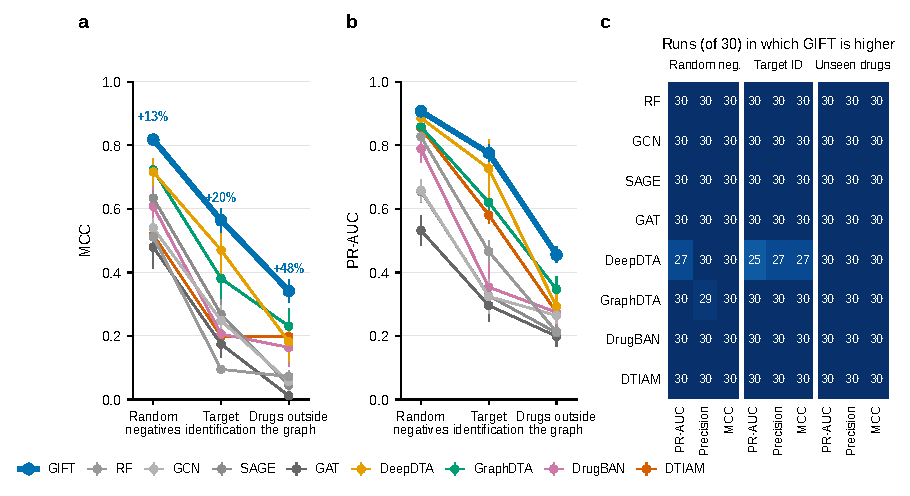
\includegraphics[width=\textwidth]{figs/dti_value_gift.pdf}
\caption{Value of GIFT for DTI prediction across the three benchmarks of increasing difficulty (30 runs). (a) MCC and (b) PR-AUC of all nine methods (mean $\pm$ s.d.); percentages: increase of GIFT's MCC over the best baseline on each benchmark. (c) Number of the 30 runs in which GIFT exceeds each baseline in PR-AUC, precision, and MCC (random neg.: ChEMBL~35 with random negatives; target ID: compound-matched negatives; unseen drugs: external benchmark).}
\label{fig:dtivalue}
\end{figure}

\begin{table*}[!t]
\centering
\caption{Held-out ChEMBL~35 interactions with random negatives (397 to 455 positives, depending on the split, and five negatives per positive whose compound has at least one potent interaction), the standard evaluation. Mean $\pm$ standard deviation over 30 training runs (seeds 42-71), each with its own random split; fixed threshold 0.5. All classifiers are trained with one negative per positive. Standard GNN: GCN, GraphSAGE, and GAT link predictors trained with the standard setup (Section~\ref{sec:evaluation}). Higher values are better; the best mean in each row is in bold. The final row counts these row-wise wins and is descriptive rather than an additional performance metric.}
\label{tab:random}
\resizebox{\textwidth}{!}{%
\begin{tabular}{l c c c c c}
\toprule
 & & & \multicolumn{3}{c}{\textbf{Standard GNN}} \\
\cmidrule(lr){4-6}
\textbf{Metric ($\uparrow$)} & \textbf{GIFT} & \textbf{Random forest} & \textbf{GCN} & \textbf{GraphSAGE} & \textbf{GAT} \\
\midrule
\multicolumn{6}{l}{\textit{Performance under class imbalance and at the decision threshold}} \\
PR-AUC & \textbf{0.907$\pm$0.010} & 0.827$\pm$0.013 & 0.658$\pm$0.034 & 0.655$\pm$0.035 & 0.532$\pm$0.046 \\
MCC & \textbf{0.818$\pm$0.019} & 0.512$\pm$0.015 & 0.540$\pm$0.030 & 0.634$\pm$0.024 & 0.480$\pm$0.067 \\
Precision & \textbf{0.859$\pm$0.032} & 0.413$\pm$0.012 & 0.459$\pm$0.035 & 0.614$\pm$0.038 & 0.398$\pm$0.052 \\
F1 & \textbf{0.848$\pm$0.016} & 0.572$\pm$0.012 & 0.604$\pm$0.028 & 0.696$\pm$0.021 & 0.550$\pm$0.053 \\
\addlinespace
\multicolumn{6}{l}{\textit{Ranking and overall classification}} \\
ROC-AUC & \textbf{0.962$\pm$0.005} & 0.939$\pm$0.006 & 0.904$\pm$0.010 & 0.911$\pm$0.008 & 0.882$\pm$0.016 \\
Per-target ROC-AUC & \textbf{0.950$\pm$0.013} & 0.930$\pm$0.013 & 0.906$\pm$0.018 & 0.914$\pm$0.015 & 0.881$\pm$0.019 \\
Accuracy & \textbf{0.950$\pm$0.006} & 0.767$\pm$0.011 & 0.805$\pm$0.025 & 0.882$\pm$0.012 & 0.745$\pm$0.085 \\
Recall & 0.838$\pm$0.023 & \textbf{0.931$\pm$0.013} & 0.889$\pm$0.021 & 0.805$\pm$0.024 & 0.905$\pm$0.021 \\
\midrule
\textbf{Metrics with best mean} & \textbf{7 of 8} & 1 of 8 & 0 of 8 & 0 of 8 & 0 of 8 \\
\bottomrule
\end{tabular}}
\end{table*}

\begin{table*}[!t]
\centering
\caption{Held-out ChEMBL~35 interactions with compound-matched negatives (the positives of Table~\ref{tab:random} and five negatives per positive involving the same compound), a stricter benchmark in which every negative involves the compound of a test interaction. Mean $\pm$ standard deviation over 30 training runs; fixed threshold 0.5. The positives, and hence the recall, are the same as in Table~\ref{tab:random}. Higher values are better; the best mean in each row is in bold. The final row counts these row-wise wins and is descriptive rather than an additional performance metric.}
\label{tab:matched}
\resizebox{\textwidth}{!}{%
\begin{tabular}{l c c c c c}
\toprule
 & & & \multicolumn{3}{c}{\textbf{Standard GNN}} \\
\cmidrule(lr){4-6}
\textbf{Metric ($\uparrow$)} & \textbf{GIFT} & \textbf{Random forest} & \textbf{GCN} & \textbf{GraphSAGE} & \textbf{GAT} \\
\midrule
\multicolumn{6}{l}{\textit{Performance under class imbalance and at the decision threshold}} \\
PR-AUC & \textbf{0.776$\pm$0.026} & 0.466$\pm$0.034 & 0.324$\pm$0.053 & 0.327$\pm$0.048 & 0.296$\pm$0.052 \\
MCC & \textbf{0.564$\pm$0.038} & 0.095$\pm$0.012 & 0.248$\pm$0.049 & 0.268$\pm$0.045 & 0.174$\pm$0.042 \\
Precision & \textbf{0.516$\pm$0.046} & 0.189$\pm$0.004 & 0.249$\pm$0.025 & 0.275$\pm$0.029 & 0.215$\pm$0.016 \\
F1 & \textbf{0.637$\pm$0.033} & 0.314$\pm$0.006 & 0.388$\pm$0.030 & 0.409$\pm$0.031 & 0.348$\pm$0.020 \\
\addlinespace
\multicolumn{6}{l}{\textit{Ranking and overall classification}} \\
ROC-AUC & \textbf{0.899$\pm$0.010} & 0.728$\pm$0.013 & 0.731$\pm$0.044 & 0.724$\pm$0.033 & 0.699$\pm$0.046 \\
Per-target ROC-AUC & \textbf{0.854$\pm$0.028} & 0.684$\pm$0.025 & 0.760$\pm$0.027 & 0.723$\pm$0.029 & 0.715$\pm$0.035 \\
Accuracy & \textbf{0.832$\pm$0.025} & 0.291$\pm$0.015 & 0.507$\pm$0.066 & 0.591$\pm$0.053 & 0.403$\pm$0.061 \\
Recall & 0.838$\pm$0.023 & \textbf{0.931$\pm$0.013} & 0.889$\pm$0.021 & 0.805$\pm$0.024 & 0.905$\pm$0.021 \\
\midrule
\textbf{Metrics with best mean} & \textbf{7 of 8} & 1 of 8 & 0 of 8 & 0 of 8 & 0 of 8 \\
\bottomrule
\end{tabular}}
\end{table*}

\begin{table*}[!t]
\centering
\caption{External compounds outside the training graph with compound-matched negatives (95 compounds; 3,243 interactions with median pChEMBL $\geq 5$ in ChEMBL~36; 15,646 negatives at proteins without a ChEMBL~36 record for the compound; 675 targets with both classes). Mean $\pm$ standard deviation over 30 training runs; fixed threshold 0.5. Pooled ROC-AUC and PR-AUC also reward ranking frequently tested targets first; the per-target ROC-AUC is unaffected by it. Higher values are better; the best mean in each row is in bold. The final row counts these row-wise wins and is descriptive rather than an additional performance metric.}
\label{tab:external}
\resizebox{\textwidth}{!}{%
\begin{tabular}{l c c c c c}
\toprule
 & & & \multicolumn{3}{c}{\textbf{Standard GNN}} \\
\cmidrule(lr){4-6}
\textbf{Metric ($\uparrow$)} & \textbf{GIFT} & \textbf{Random forest} & \textbf{GCN} & \textbf{GraphSAGE} & \textbf{GAT} \\
\midrule
\multicolumn{6}{l}{\textit{Performance under class imbalance and at the decision threshold}} \\
PR-AUC & \textbf{0.456$\pm$0.026} & 0.213$\pm$0.007 & 0.264$\pm$0.026 & 0.210$\pm$0.019 & 0.199$\pm$0.031 \\
MCC & \textbf{0.342$\pm$0.037} & 0.072$\pm$0.021 & 0.057$\pm$0.035 & 0.045$\pm$0.031 & 0.012$\pm$0.066 \\
Precision & \textbf{0.673$\pm$0.034} & 0.241$\pm$0.021 & 0.259$\pm$0.052 & 0.212$\pm$0.031 & 0.187$\pm$0.052 \\
F1 & \textbf{0.357$\pm$0.050} & 0.211$\pm$0.025 & 0.128$\pm$0.047 & 0.206$\pm$0.044 & 0.183$\pm$0.051 \\
\addlinespace
\multicolumn{6}{l}{\textit{Ranking and recovery}} \\
ROC-AUC & \textbf{0.725$\pm$0.021} & 0.561$\pm$0.010 & 0.692$\pm$0.025 & 0.608$\pm$0.029 & 0.591$\pm$0.064 \\
Per-target ROC-AUC & \textbf{0.618$\pm$0.014} & 0.558$\pm$0.009 & 0.546$\pm$0.027 & 0.563$\pm$0.017 & 0.549$\pm$0.016 \\
Recall & \textbf{0.245$\pm$0.047} & 0.190$\pm$0.036 & 0.089$\pm$0.042 & 0.219$\pm$0.084 & 0.198$\pm$0.081 \\
\midrule
\textbf{Metrics with best mean} & \textbf{7 of 7} & 0 of 7 & 0 of 7 & 0 of 7 & 0 of 7 \\
\bottomrule
\end{tabular}}
\end{table*}

\begin{table*}[!t]
\centering
\caption{Comparison with DeepDTA, GraphDTA (GIN variant), DrugBAN (official implementation), and DTIAM (official implementation; $^{\dagger}$frozen pretrained encoders, interaction head trained in every run) on the three benchmarks of Tables~\ref{tab:random}, \ref{tab:matched}, and~\ref{tab:external}. DeepDTA, GraphDTA, and DrugBAN are trained with their standard configurations from scratch as binary classifiers on the ChEMBL~35 training interactions of each run, with the same training negatives, validation set, and fixed threshold of 0.5 as GIFT. Mean $\pm$ standard deviation over the same 30 runs. The last column gives the number of the 30 runs in which GIFT is better than DeepDTA (D), GraphDTA (G), DrugBAN (B), and DTIAM (T); for example, ``D: 20, G: 8'' means better than DeepDTA in 20 runs and better than GraphDTA in 8 runs. FP, false positives; total errors, false positives plus false negatives. Best mean in each row in bold.}
\label{tab:dta}
\resizebox{\textwidth}{!}{%
\begin{tabular}{l c c c c c c}
\toprule
\textbf{Metric} & \textbf{GIFT} & \textbf{DeepDTA} & \textbf{GraphDTA} & \textbf{DrugBAN} & \textbf{DTIAM}$^{\dagger}$ & \textbf{Runs GIFT better (of 30)} \\
\midrule
\multicolumn{7}{l}{\textit{ChEMBL~35, random negatives}} \\
PR-AUC $\uparrow$ & \textbf{0.907$\pm$0.010} & 0.886$\pm$0.026 & 0.858$\pm$0.022 & 0.789$\pm$0.042 & 0.854$\pm$0.014 & D: 27, G: 30, B: 30, T: 30 \\
MCC $\uparrow$ & \textbf{0.818$\pm$0.019} & 0.716$\pm$0.043 & 0.723$\pm$0.036 & 0.608$\pm$0.081 & 0.519$\pm$0.023 & D: 30, G: 30, B: 30, T: 30 \\
Precision $\uparrow$ & \textbf{0.859$\pm$0.032} & 0.662$\pm$0.065 & 0.716$\pm$0.066 & 0.528$\pm$0.099 & 0.412$\pm$0.023 & D: 30, G: 29, B: 30, T: 30 \\
F1 $\uparrow$ & \textbf{0.848$\pm$0.016} & 0.760$\pm$0.039 & 0.769$\pm$0.031 & 0.661$\pm$0.075 & 0.574$\pm$0.021 & D: 30, G: 30, B: 30, T: 30 \\
ROC-AUC $\uparrow$ & 0.962$\pm$0.005 & \textbf{0.963$\pm$0.006} & 0.950$\pm$0.007 & 0.943$\pm$0.012 & 0.949$\pm$0.006 & D: 11, G: 29, B: 30, T: 30 \\
Per-target ROC-AUC $\uparrow$ & \textbf{0.950$\pm$0.013} & 0.946$\pm$0.013 & 0.936$\pm$0.016 & 0.925$\pm$0.018 & 0.938$\pm$0.012 & D: 19, G: 27, B: 29, T: 24 \\
Recall $\uparrow$ & 0.838$\pm$0.023 & 0.898$\pm$0.021 & 0.836$\pm$0.029 & 0.911$\pm$0.035 & \textbf{0.948$\pm$0.013} & D: 0, G: 14, B: 1, T: 0 \\
FP $\downarrow$ & \textbf{59.8$\pm$16.2} & 204.7$\pm$66.8 & 149.0$\pm$55.1 & 386.5$\pm$190.4 & 586.7$\pm$63.5 & D: 30, G: 29, B: 30, T: 30 \\
Total errors $\downarrow$ & \textbf{129.9$\pm$14.1} & 248.9$\pm$61.3 & 219.7$\pm$46.9 & 425.2$\pm$180.1 & 609.3$\pm$60.7 & D: 30, G: 30, B: 30, T: 30 \\
\textit{Metrics with best mean} & \textbf{7 of 9} & 1 of 9 & 0 of 9 & 0 of 9 & 1 of 9 & \\
\midrule
\multicolumn{7}{l}{\textit{ChEMBL~35, compound-matched negatives}} \\
PR-AUC $\uparrow$ & \textbf{0.776$\pm$0.026} & 0.727$\pm$0.091 & 0.621$\pm$0.056 & 0.354$\pm$0.086 & 0.581$\pm$0.025 & D: 25, G: 30, B: 30, T: 30 \\
MCC $\uparrow$ & \textbf{0.564$\pm$0.038} & 0.470$\pm$0.102 & 0.381$\pm$0.078 & 0.206$\pm$0.059 & 0.199$\pm$0.022 & D: 27, G: 30, B: 30, T: 30 \\
Precision $\uparrow$ & \textbf{0.516$\pm$0.046} & 0.405$\pm$0.083 & 0.349$\pm$0.067 & 0.228$\pm$0.028 & 0.217$\pm$0.009 & D: 27, G: 30, B: 30, T: 30 \\
F1 $\uparrow$ & \textbf{0.637$\pm$0.033} & 0.552$\pm$0.081 & 0.488$\pm$0.062 & 0.364$\pm$0.033 & 0.353$\pm$0.011 & D: 27, G: 30, B: 30, T: 30 \\
ROC-AUC $\uparrow$ & \textbf{0.899$\pm$0.010} & 0.893$\pm$0.050 & 0.838$\pm$0.024 & 0.731$\pm$0.056 & 0.797$\pm$0.015 & D: 10, G: 30, B: 30, T: 30 \\
Per-target ROC-AUC $\uparrow$ & \textbf{0.854$\pm$0.028} & 0.851$\pm$0.060 & 0.761$\pm$0.040 & 0.694$\pm$0.050 & 0.727$\pm$0.025 & D: 12, G: 30, B: 30, T: 30 \\
Recall $\uparrow$ & 0.838$\pm$0.023 & 0.898$\pm$0.021 & 0.836$\pm$0.029 & 0.911$\pm$0.035 & \textbf{0.948$\pm$0.013} & D: 0, G: 14, B: 1, T: 0 \\
FP $\downarrow$ & \textbf{344.7$\pm$64.6} & 623.5$\pm$269.7 & 715.8$\pm$231.2 & 1,356.7$\pm$241.6 & 1,479.6$\pm$91.4 & D: 27, G: 29, B: 30, T: 30 \\
Total errors $\downarrow$ & \textbf{414.7$\pm$59.9} & 667.7$\pm$264.7 & 786.5$\pm$221.9 & 1,395.4$\pm$230.4 & 1,502.2$\pm$88.9 & D: 27, G: 30, B: 30, T: 30 \\
\textit{Metrics with best mean} & \textbf{8 of 9} & 0 of 9 & 0 of 9 & 0 of 9 & 1 of 9 & \\
\midrule
\multicolumn{7}{l}{\textit{External compounds (ChEMBL~36), compound-matched negatives}} \\
PR-AUC $\uparrow$ & \textbf{0.456$\pm$0.026} & 0.293$\pm$0.048 & 0.347$\pm$0.039 & 0.274$\pm$0.045 & 0.275$\pm$0.018 & D: 30, G: 30, B: 30, T: 30 \\
MCC $\uparrow$ & \textbf{0.342$\pm$0.037} & 0.182$\pm$0.063 & 0.231$\pm$0.055 & 0.164$\pm$0.059 & 0.198$\pm$0.027 & D: 30, G: 30, B: 30, T: 30 \\
Precision $\uparrow$ & \textbf{0.673$\pm$0.034} & 0.401$\pm$0.079 & 0.385$\pm$0.059 & 0.276$\pm$0.050 & 0.249$\pm$0.017 & D: 30, G: 30, B: 30, T: 30 \\
F1 $\uparrow$ & 0.357$\pm$0.050 & 0.259$\pm$0.070 & 0.348$\pm$0.054 & 0.336$\pm$0.038 & \textbf{0.367$\pm$0.017} & D: 27, G: 15, B: 21, T: 14 \\
ROC-AUC $\uparrow$ & \textbf{0.725$\pm$0.021} & 0.608$\pm$0.056 & 0.667$\pm$0.026 & 0.636$\pm$0.041 & 0.664$\pm$0.020 & D: 30, G: 30, B: 29, T: 30 \\
Per-target ROC-AUC $\uparrow$ & \textbf{0.618$\pm$0.014} & 0.589$\pm$0.026 & 0.563$\pm$0.019 & 0.569$\pm$0.024 & 0.601$\pm$0.011 & D: 26, G: 30, B: 29, T: 25 \\
Recall $\uparrow$ & 0.245$\pm$0.047 & 0.202$\pm$0.080 & 0.330$\pm$0.083 & 0.448$\pm$0.077 & \textbf{0.706$\pm$0.053} & D: 20, G: 7, B: 1, T: 0 \\
FP $\downarrow$ & \textbf{391.0$\pm$103.3} & 1,033.4$\pm$504.5 & 1,788.5$\pm$718.3 & 4,031.9$\pm$1,559.7 & 6,974.8$\pm$945.7 & D: 30, G: 30, B: 30, T: 30 \\
Total errors $\downarrow$ & \textbf{2,838.8$\pm$91.0} & 3,620.8$\pm$380.1 & 3,960.1$\pm$555.2 & 5,823.1$\pm$1,372.3 & 7,927.1$\pm$812.3 & D: 30, G: 30, B: 30, T: 30 \\
\textit{Metrics with best mean} & \textbf{7 of 9} & 0 of 9 & 0 of 9 & 0 of 9 & 2 of 9 & \\
\bottomrule
\end{tabular}}
\end{table*}

\begin{table*}[!t]
\centering
\caption{Confusion-matrix counts at the fixed threshold of 0.5 for the three classification benchmarks, organized to distinguish incorrect from correct predictions. Values are mean $\pm$ standard deviation over 30 runs and are therefore not necessarily integers. Total errors are FP$+$FN. The ChEMBL~35 test-set sizes vary with the random split, whereas the external benchmark contains 3,243 positives and 15,646 negatives in every run. TP, true positives; FN, false negatives; FP, false positives; TN, true negatives. DeepDTA, GraphDTA, and DrugBAN use their standard configurations, and DTIAM$^{\dagger}$ its frozen pretrained encoders with its official interaction head trained in every run (Section~\ref{sec:evaluation}). Arrows indicate the favorable direction, and the best mean within each benchmark and column is in bold.}
\label{tab:confusion}
\resizebox{\textwidth}{!}{%
\begin{tabular}{l l r r r r r}
\toprule
\textbf{Benchmark} & \textbf{Method} & \multicolumn{3}{c}{\textbf{Incorrect predictions}} & \multicolumn{2}{c}{\textbf{Correct predictions}} \\
\cmidrule(lr){3-5}\cmidrule(lr){6-7}
 & & \textbf{FP $\downarrow$} & \textbf{FN $\downarrow$} & \textbf{Total errors $\downarrow$} & \textbf{TP $\uparrow$} & \textbf{TN $\uparrow$} \\
\midrule
\multirow{9}{*}{ChEMBL~35, random negatives}
 & \textbf{GIFT} & \textbf{59.8$\pm$16.2} & 70.1$\pm$10.6 & \textbf{129.9$\pm$14.1} & 361.5$\pm$15.3 & \textbf{2,098.2$\pm$78.9} \\
 & Random forest & 572.4$\pm$37.0 & 29.8$\pm$5.7 & 602.2$\pm$36.8 & 401.8$\pm$15.2 & 1,585.6$\pm$60.7 \\
 & GCN & 458.5$\pm$73.9 & 47.9$\pm$9.3 & 506.5$\pm$69.2 & 383.7$\pm$16.5 & 1,699.5$\pm$85.9 \\
 & GraphSAGE & 221.4$\pm$39.5 & 84.0$\pm$10.3 & 305.4$\pm$35.1 & 347.6$\pm$17.0 & 1,936.6$\pm$72.1 \\
 & GAT & 616.3$\pm$212.9 & 40.9$\pm$9.2 & 657.2$\pm$205.2 & 390.7$\pm$15.0 & 1,541.7$\pm$240.6 \\
 & DeepDTA & 204.7$\pm$66.8 & 44.2$\pm$8.9 & 248.9$\pm$61.3 & 387.4$\pm$16.4 & 1,953.3$\pm$86.1 \\
 & GraphDTA & 149.0$\pm$55.1 & 70.7$\pm$12.5 & 219.7$\pm$46.9 & 360.9$\pm$19.2 & 2,009.0$\pm$70.7 \\
 & DrugBAN & 386.5$\pm$190.4 & 38.7$\pm$15.3 & 425.2$\pm$180.1 & 392.9$\pm$19.1 & 1,771.5$\pm$189.8 \\
 & DTIAM$^{\dagger}$ & 586.7$\pm$63.5 & \textbf{22.6$\pm$5.8} & 609.3$\pm$60.7 & \textbf{409.0$\pm$15.4} & 1,571.3$\pm$80.6 \\
\midrule
\multirow{9}{*}{ChEMBL~35, compound-matched}
 & \textbf{GIFT} & \textbf{344.7$\pm$64.6} & 70.1$\pm$10.6 & \textbf{414.7$\pm$59.9} & 361.5$\pm$15.3 & \textbf{1,697.5$\pm$88.9} \\
 & Random forest & 1,723.2$\pm$61.9 & 29.8$\pm$5.7 & 1,753.0$\pm$60.5 & 401.8$\pm$15.2 & 319.0$\pm$40.1 \\
 & GCN & 1,172.5$\pm$172.5 & 47.9$\pm$9.3 & 1,220.5$\pm$168.1 & 383.7$\pm$16.5 & 869.7$\pm$169.9 \\
 & GraphSAGE & 928.8$\pm$142.4 & 84.0$\pm$10.3 & 1,012.8$\pm$138.6 & 347.6$\pm$17.0 & 1,113.4$\pm$132.7 \\
 & GAT & 1,433.1$\pm$146.2 & 40.9$\pm$9.2 & 1,474.0$\pm$139.9 & 390.7$\pm$15.0 & 609.1$\pm$164.7 \\
 & DeepDTA & 623.5$\pm$269.7 & 44.2$\pm$8.9 & 667.7$\pm$264.7 & 387.4$\pm$16.4 & 1,418.7$\pm$268.7 \\
 & GraphDTA & 715.8$\pm$231.2 & 70.7$\pm$12.5 & 786.5$\pm$221.9 & 360.9$\pm$19.2 & 1,326.4$\pm$213.3 \\
 & DrugBAN & 1,356.7$\pm$241.6 & 38.7$\pm$15.3 & 1,395.4$\pm$230.4 & 392.9$\pm$19.1 & 685.5$\pm$234.6 \\
 & DTIAM$^{\dagger}$ & 1,479.6$\pm$91.4 & \textbf{22.6$\pm$5.8} & 1,502.2$\pm$88.9 & \textbf{409.0$\pm$15.4} & 562.6$\pm$84.6 \\
\midrule
\multirow{9}{*}{External ChEMBL~36}
 & \textbf{GIFT} & \textbf{391.0$\pm$103.3} & 2,447.9$\pm$151.5 & \textbf{2,838.8$\pm$91.0} & 795.1$\pm$151.5 & \textbf{15,255.0$\pm$103.3} \\
 & Random forest & 1,953.0$\pm$376.7 & 2,626.6$\pm$115.4 & 4,579.6$\pm$286.6 & 616.4$\pm$115.4 & 13,693.0$\pm$376.7 \\
 & GCN & 825.4$\pm$338.2 & 2,954.1$\pm$136.8 & 3,779.5$\pm$232.0 & 288.9$\pm$136.8 & 14,820.6$\pm$338.2 \\
 & GraphSAGE & 2,736.2$\pm$1,151.8 & 2,531.3$\pm$273.4 & 5,267.5$\pm$904.9 & 711.7$\pm$273.4 & 12,909.8$\pm$1,151.8 \\
 & GAT & 2,984.1$\pm$1,521.5 & 2,600.2$\pm$261.8 & 5,584.4$\pm$1,358.4 & 642.8$\pm$261.8 & 12,661.9$\pm$1,521.5 \\
 & DeepDTA & 1,033.4$\pm$504.5 & 2,587.4$\pm$260.0 & 3,620.8$\pm$380.1 & 655.6$\pm$260.0 & 14,612.6$\pm$504.5 \\
 & GraphDTA & 1,788.5$\pm$718.3 & 2,171.6$\pm$270.0 & 3,960.1$\pm$555.2 & 1,071.4$\pm$270.0 & 13,857.5$\pm$718.3 \\
 & DrugBAN & 4,031.9$\pm$1,559.7 & 1,791.3$\pm$249.4 & 5,823.1$\pm$1,372.3 & 1,451.7$\pm$249.4 & 11,614.1$\pm$1,559.7 \\
 & DTIAM$^{\dagger}$ & 6,974.8$\pm$945.7 & \textbf{952.3$\pm$171.6} & 7,927.1$\pm$812.3 & \textbf{2,290.7$\pm$171.6} & 8,671.2$\pm$945.7 \\
\bottomrule
\end{tabular}}
\end{table*}

\paragraph{Error-count comparison}
GIFT has the fewest total classification errors of all nine methods in all three benchmarks (Table~\ref{tab:confusion}). On the standard ChEMBL~35 benchmark, the random forest, GCN, and GAT recover 22 to 40 more positives per run than GIFT, but produce 399 to 557 more false positives. Even relative to GraphSAGE, the most selective standard GNN, GIFT produces 73\% fewer false positives (59.8 vs.\ 221.4) and 57\% fewer total errors (129.9 vs.\ 305.4). The distinction becomes stronger in target identification with compound-matched negatives: GIFT makes 415 total errors per run, compared with 1,013 to 1,753 for the random forest and the standard GNNs, as it limits false positives to 345 while retaining 362 true positives. Thus, the higher recall of several baselines is obtained by labeling a much larger fraction of negative pairs as interactions, whereas GIFT's higher precision and MCC reflect substantially better control of false discoveries. On the external benchmark, GIFT has more true positives than the random forest and the standard GNNs (795 vs.\ 289-712), the fewest false positives (391 vs.\ 825-2,984), and the fewest total errors (2,839 vs.\ 3,780-5,584). Its external advantage is therefore not produced by conservative prediction alone: it recovers more previously unseen interactions while making fewer incorrect positive calls. DeepDTA and GraphDTA, the most competitive baselines on ChEMBL~35, produce 2.5 to 3.4 times as many false positives as GIFT with random negatives (149.0 to 204.7, compared with 59.8) and 1.8 to 2.1 times as many with compound-matched negatives (623.5 to 715.8, compared with 344.7), and therefore 1.6 to 1.9 times as many total errors on both ChEMBL~35 benchmarks. On the external compounds, GraphDTA recovers more interactions than GIFT (1,071.4 true positives, compared with 795.1), but at the cost of 4.6 times as many false positives (1,788.5, compared with 391.0) and 1.4 times as many total errors (3,960.1, compared with 2,838.8). These error patterns explain why PR-AUC, precision, and MCC provide stronger evidence of useful target identification than recall considered in isolation.

\subsubsection{Errors Concentrate on Proteins Without Training Interactions}
\label{sec:misclassification}

To characterize the failure modes on ChEMBL~35, the misclassifications of the model of the run with seed 42 on the standard benchmark with random negatives ($|\mathcal{D}_{test}| = 2{,}658$: 443 positives and 2,215 negatives) were analyzed at the fixed threshold of 0.5:

\begin{itemize}
    \item \textbf{Overall performance:} accuracy = 0.954 and F1-score = 0.864, with a recall of 0.867 and a precision of 0.861.
    \item \textbf{False positives:} 62, that is, 2.3\% of the test pairs and a false positive rate of 2.8\% (62 of the 2,215 negatives).
    \item \textbf{False negatives:} 59, that is, 2.2\% of the test pairs and a false negative rate of 13.3\% (59 of the 443 positives).
\end{itemize}

The model classifies 95.4\% of the test pairs correctly, including 97.2\% of the negatives and 86.7\% of the positives, and 86.1\% of its predicted interactions are held-out interactions. It makes about a fifth as many errors as the random forest of the same run on the same pairs (121, compared with 581), as it produces far fewer false positives (62, compared with 549), at the cost of more false negatives (59, compared with 32). Its errors are about equally often false positives and false negatives: it rarely predicts an interaction for a random pair, and misses about one in eight held-out interactions.

\paragraph{Misclassified pairs, compounds, and proteins}
The compound-protein pairs, compounds, and proteins with the most misclassifications are summarized below:
\begin{itemize}
    \item \textbf{Compound-protein pairs:} 121 pairs (4.6\% of 2,658 test pairs) are misclassified. Most errors are confident rather than borderline: 83 of them have a score below 0.1 or above 0.9, and 8 lie between 0.4 and 0.6. The most confident false negatives include silvestrol (CHEMBL555196) at eukaryotic initiation factor 4A-I (CHEMBL2052028), paclitaxel (CHEMBL428647) at tyrosine-protein kinase Mer (CHEMBL5331), and piplartine (CHEMBL465843) at signal transducer and activator of transcription 3 (CHEMBL4026); the most confident false positives include three unnamed compounds (CHEMBL440877, CHEMBL82546, and CHEMBL196185) at the glucocorticoid receptor (CHEMBL3368), doxorubicin hydrochloride (CHEMBL359744) at DNA topoisomerase 2-alpha (CHEMBL3586), the established target of doxorubicin, tozasertib (CHEMBL572878) at serine/threonine-protein kinase VRK1 (CHEMBL1293199), sunitinib (CHEMBL535) at transcription factor p65 (CHEMBL5533), and midostaurin (CHEMBL608533) at cell division cycle 7-related protein kinase (CHEMBL5443), all with scores above 0.99.

    \item \textbf{Compounds:} 67 of the 216 compounds in the benchmark have at least one misclassified pair. The most frequently misclassified compounds are bortezomib (CHEMBL325041; five of its seven positives missed and one false positive) and podofilox (CHEMBL61; all five positives missed), followed by four compounds with four errors each: colchicine (CHEMBL107; two of its five positives missed and two false positives), sunitinib (CHEMBL535; four false positives, out of 47 test positives), RG-1530 (CHEMBL1980391; four false positives, out of 20 test positives), and doxorubicin hydrochloride (CHEMBL359744; all three positives missed and one false positive).

    \item \textbf{Proteins:} 109 of the 1,160 proteins in the benchmark have at least one misclassified pair, and none has more than three.
\end{itemize}

The misclassification analysis reveals two systematic patterns. First, the false negatives concentrate on proteins without training evidence: the model misses 31 of the 51 positives (61\%) at proteins without training interactions, compared with 28 of the 392 (7\%) at proteins with at least one; missed positives also involve compounds with fewer training interactions than recovered ones (median 9 vs.\ 60). Second, 61 of the 62 false positives involve a compound with training interactions, as do most negatives of this benchmark (1,937 of the 2,215), and the compounds with the most false positives, RG-1530 and sunitinib, have many test positives (20 and 47). Since negatives are pairs without recorded activity, some of these false positives may be activities that have not been tested or recorded, such as doxorubicin at DNA topoisomerase 2-alpha. When every negative involves a test compound, as in the compound-matched benchmark (Table~\ref{tab:matched}), false positives become the main error (355 of 2,075 negatives). In the pair embedding of the encoder (Figure~\ref{fig:tsne_pred}), part of the pairs whose protein has no training interactions forms a separate group of 204 pairs, all involving such a protein, which contains 10 of the 443 positives, 9 of them missed. The remaining errors (50 of the 59 false negatives and 59 of the 62 false positives) lie among pairs of the other class: the false positives mostly among positives and the false negatives mostly among negatives.

\begin{figure}[!htbp]
\centering
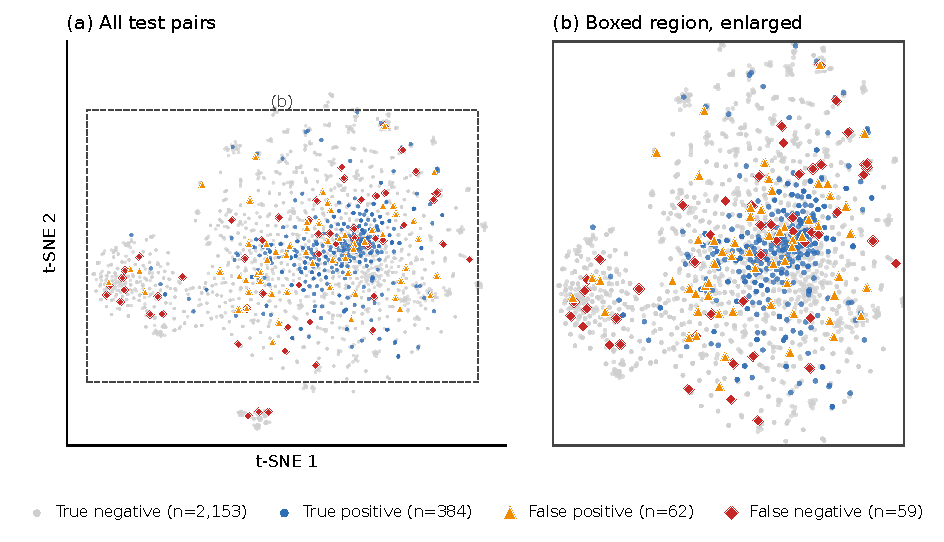
\includegraphics[width=0.75\textwidth]{figs/tsne_pairs_predictions.pdf}
\caption{t-SNE of the ChEMBL~35 test pairs with random negatives (seed 42) in the pair embedding $u_{cp}$ of the trained encoder (128 dimensions), colored by the outcome at the fixed threshold of 0.5: true negatives (grey, n=2,153), true positives (blue, n=384), false positives (triangles, n=62), and false negatives (diamonds, n=59). (a) All test pairs; (b) the boxed region, enlarged. The group at the far left contains 204 pairs, all involving a protein without training interactions; the boxed region contains 440 of the 443 positives, 56 of the 59 false negatives, and all 62 false positives. In the 128-dimensional embedding, 69\% of the ten nearest neighbors of a positive are positives and 70\% of those of a negative are negatives; 54\% of the neighbors of the false positives are true positives, and 56\% of those of the false negatives are true negatives.}
\label{fig:tsne_pred}
\end{figure}

\subsection{Known Actives Are Enriched at the Top of the Per-Target Rankings}
\label{sec:leadprio}

\begin{figure}[!t]
\centering
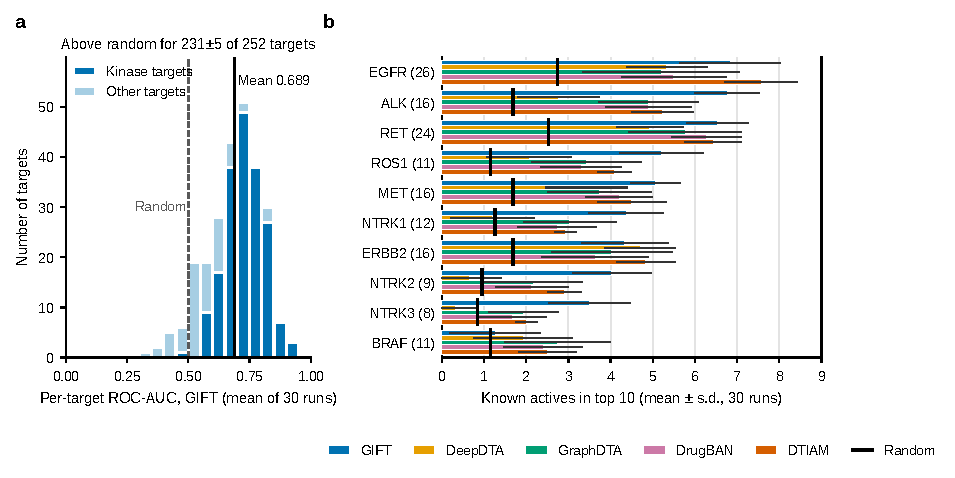
\includegraphics[width=0.8\textwidth]{figs/lead_prioritization_gift.pdf}
\caption{Compound prioritization of the 95 external drugs. (a) Per-target ROC-AUC of GIFT, averaged over the 30 runs, for the 252 targets with at least five known actives; dashed: random; solid: mean; title: targets above random per run (mean $\pm$ s.d.). (b) Known actives in the top 10 per driver kinase ($n$ in parentheses) for GIFT, DeepDTA, GraphDTA, DrugBAN, and DTIAM; bars: mean $\pm$ s.d. over 30 runs; ticks: random.}
\label{fig:leadprio}
\end{figure}

For drug prioritization, the model concentrates known actives at the top of the per-target rankings: for the ten driver kinases, nearly half of its 10 top-ranked drugs are known actives ($4.8\pm0.4$ of 10, 3.1 times the random expectation), and across 252 targets the rankings carry target-specific information beyond the protein family. For the individual driver kinases, however, the enrichment is largely shared across the kinase family.

\paragraph{All targets}
Across the 252 targets with at least five known actives among the 95 external compounds, the rankings place the known actives above the other compounds for $231\pm5$ targets (ROC-AUC $>0.5$), with a ROC-AUC of at least 0.7 for $132\pm23$ targets (mean $0.689\pm0.019$, median $0.706\pm0.025$), and for $226\pm12$ targets at least one known active is among the 10 top-ranked compounds. On average, $2.26\pm0.28$ known actives are among the 10 top-ranked compounds, 2.3 times the random expectation (0.99). Beyond the protein family, the rankings also carry target-specific information: they exceed the model's own family ranking for $176\pm22$ of the 252 targets (mean ROC-AUC 0.689 vs.\ 0.662; Wilcoxon $p<0.05$ in 29 of the 30 runs) and, within the kinase family, for $129\pm22$ of the 189 kinase targets (0.731 vs.\ 0.712; $p<0.01$ in 26 of the 30 runs), and they exceed its global ranking for $230\pm7$ targets (0.689 vs.\ 0.614).

\paragraph{Driver kinases of non-small cell lung cancer}
In a repurposing setting, the task is to select, from a set of clinical-stage drugs, those most likely to act on a given target. For the ten driver kinases (Figure~2b of the main text, Table~\ref{tab:leadprio}), the model places on average $4.8\pm0.4$ known actives among its 10 top-ranked compounds, 3.1 times the random expectation (1.6), with a mean ROC-AUC of $0.780\pm0.024$. For every driver kinase, it ranks the known actives above the other compounds on average over the 30 runs (mean ROC-AUC 0.65 for BRAF to 0.84 for NTRK2), and its 10 top-ranked compounds contain more known actives than expected at random for nine of the ten driver kinases in 19 runs and for all ten in 11; the exception is BRAF ($1.3\pm1.1$ known actives among the 10 top-ranked compounds, 1.2 expected). In the run with seed 42, approved kinase inhibitors are ranked highly for targets at which they are potent: the ALK and ROS1 inhibitor ceritinib is ranked first for ROS1 (median pChEMBL 8.7), ALK (8.0), RET (6.0), MET (5.9), NTRK2 (5.7), and NTRK1 (5.6), and afatinib is ranked second for ERBB2 (7.5) and EGFR (8.7). Afatinib, ranked fourth for RET and fifth for MET, has no known activity at these kinases in the external set, but ChEMBL~37 reports pChEMBL values of 5.4 and 6.8 for its parent compound, which were not captured since the external set contains the dimaleate salt.

\begin{table*}[!t]
\centering
\caption{Drug prioritization for the actionable driver kinases of non-small cell lung cancer among the 95 external compounds. $n$: known actives (median pChEMBL $\geq 5$ in ChEMBL~36). ROC-AUC and known actives in top 10: mean $\pm$ standard deviation over 30 training runs. Random: expected number of known actives among 10 compounds drawn at random. Top-ranked compounds: the three highest-ranked compounds in the run with seed 42. Mean rows: per-target rankings, or the same compound ranking for every driver kinase ordered by the mean score over all kinases (UniProt keyword Kinase; family) or over all graph proteins (global). $^{*}$known active; $^{\dagger}$pChEMBL $\geq 5$ reported for the parent compound in ChEMBL~37 but absent from the external set; $^{\ddagger}$activity records in ChEMBL~37, none with pChEMBL $\geq 5$; no mark: no activity record.}
\label{tab:leadprio}
\resizebox{\textwidth}{!}{%
\begin{tabular}{l c c c c l}
\toprule
 & & & \multicolumn{2}{c}{\textbf{Known actives in top 10}} & \\
\cmidrule(lr){4-5}
\textbf{Target} & $n$ & \textbf{ROC-AUC} & GIFT & Random & \textbf{Top-ranked compounds (seed 42)} \\
\midrule
EGFR & 26 & 0.72$\pm$0.05 & 6.8$\pm$1.2 & 2.7 & Palbociclib$^{\ddagger}$, Afatinib$^{*}$, Gilteritinib$^{*}$ \\
RET & 24 & 0.76$\pm$0.03 & 6.5$\pm$0.7 & 2.5 & Ceritinib$^{*}$, Repotrectinib, Dacomitinib$^{\ddagger}$ \\
ERBB2 & 16 & 0.74$\pm$0.05 & 4.3$\pm$1.0 & 1.7 & Ceritinib, Afatinib$^{*}$, Neratinib$^{*}$ \\
MET & 16 & 0.81$\pm$0.04 & 5.1$\pm$0.6 & 1.7 & Ceritinib$^{*}$, Repotrectinib, Entrectinib$^{*}$ \\
ALK & 16 & 0.83$\pm$0.04 & 6.8$\pm$0.8 & 1.7 & Ceritinib$^{*}$, Afatinib$^{\ddagger}$, Repotrectinib$^{*}$ \\
NTRK1 & 12 & 0.80$\pm$0.04 & 4.4$\pm$0.9 & 1.3 & Ceritinib$^{*}$, Repotrectinib$^{*}$, Afatinib$^{\ddagger}$ \\
BRAF & 11 & 0.65$\pm$0.05 & 1.3$\pm$1.1 & 1.2 & Ceritinib$^{\ddagger}$, Afatinib$^{\ddagger}$, Lapatinib$^{\ddagger}$ \\
ROS1 & 11 & 0.83$\pm$0.04 & 5.2$\pm$1.0 & 1.2 & Ceritinib$^{*}$, Dacomitinib, Lapatinib$^{\ddagger}$ \\
NTRK2 & 9 & 0.84$\pm$0.04 & 4.0$\pm$0.9 & 0.9 & Ceritinib$^{*}$, Repotrectinib$^{*}$, Nintedanib$^{*}$ \\
NTRK3 & 8 & 0.83$\pm$0.04 & 3.5$\pm$1.0 & 0.8 & Ceritinib, Gilteritinib, Repotrectinib$^{*}$ \\
\midrule
\multicolumn{2}{l}{Mean, per target} & 0.78$\pm$0.02 & 4.8$\pm$0.4 & 1.6 & \\
\multicolumn{2}{l}{Mean, family} & 0.76$\pm$0.02 & 4.5$\pm$0.4 & 1.6 & \\
\multicolumn{2}{l}{Mean, global} & 0.71$\pm$0.03 & 4.5$\pm$0.4 & 1.6 & \\
\bottomrule
\end{tabular}}
\end{table*}

\paragraph{Selectivity between driver kinases}
This enrichment is achieved largely at the level of the kinase family. The model's kinase-family ranking, which gives every driver kinase the same compound ranking, places nearly as many known actives among the 10 top-ranked compounds of the driver kinases ($4.5\pm0.4$) as its per-target rankings ($4.8\pm0.4$), at a lower ROC-AUC ($0.755\pm0.024$ compared with $0.780\pm0.024$; Table~\ref{tab:leadprio}). Accordingly, the top-ranked compounds are the same few multi-kinase inhibitors (in the run with seed 42, ceritinib, afatinib, and repotrectinib) for most driver kinases. For the 38 compounds that are active at some but not all of the ten driver kinases, the model ranks the kinases at which they are active only moderately above the others (cross-target ROC-AUC $0.61\pm0.04$). Restricted to drugs with recorded activities at each driver kinase (22 to 81 per kinase), which are mostly kinase inhibitors, it separates actives from tested inactives with a mean ROC-AUC of $0.62\pm0.03$, close to its kinase-family ranking ($0.60\pm0.03$); for BRAF, it ranks tested inactives above actives in 28 of the 30 runs (ROC-AUC 0.27 to 0.53). In a repurposing screen, the model therefore separates kinase inhibitors from drugs of many other therapeutic classes, the first step in prioritizing candidates for a kinase target; separating the individual driver kinases remains an open challenge.

\paragraph{Top-ranked candidates}
Figure~2a of the main text shows the 12 drugs that the model of the run with seed 42 ranks among the five highest for at least one driver kinase, with the recorded evidence for every drug-kinase pair. Of its 50 top-five picks (five per driver kinase), 26 are active at the corresponding kinase (24 known actives and 2 actives recorded only for the parent compound), 3.3 times the 7.8 expected at random; 15 have activity records without pChEMBL $\geq 5$, and 9 have no record. Six of the ten first-ranked picks are actives. Over the 30 runs, $25.6\pm3.6$ of the 50 top-five picks and $6.8\pm0.9$ of the ten first-ranked picks are actives. Ceritinib, an approved inhibitor of ALK and ROS1, is ranked first for nine of the ten driver kinases, all except EGFR, and is active at six of these nine; entrectinib is active at all four of its top-five placements, neratinib at all three, and nintedanib at both of its two, and the BRAF inhibitor vemurafenib is ranked fourth for BRAF, at which it is active. Afatinib is ranked among the top five for eight driver kinases and is active at four of them (two of the activities are recorded only for its parent compound), and repotrectinib is ranked among the top five for eight driver kinases and is active at four of them, whereas dacomitinib is active at only one of its five top-five placements and the CDK4/6 inhibitor palbociclib and lapatinib at none of their three, which illustrates the limited selectivity between kinases. For EGFR, palbociclib is ranked first, with 26 activity records at EGFR, none with pChEMBL $\geq 5$, and epinephrine, a drug of another therapeutic class, is ranked fourth, with two activity records at EGFR, neither potent. The nine top-five picks without any activity record, ceritinib at ERBB2 and NTRK3, repotrectinib at ERBB2, RET, MET, and BRAF, dacomitinib at ALK and ROS1, and gilteritinib at NTRK3, are untested; given the limited selectivity, they are hypotheses of kinase activity rather than target-specific predictions.

\begin{figure}[!htbp]
\centering
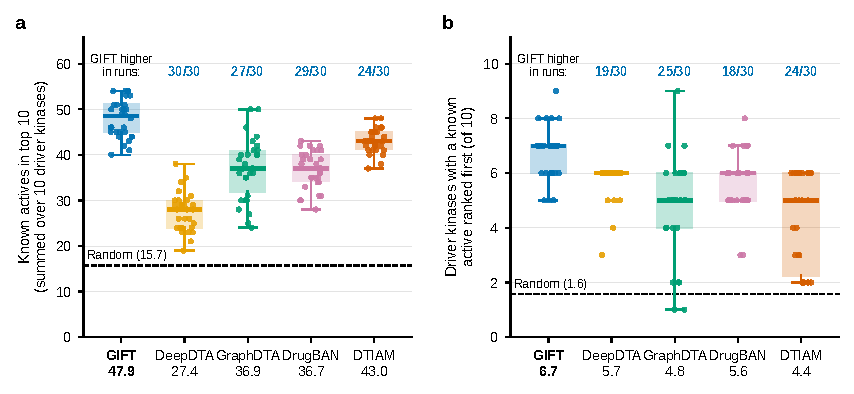
\includegraphics[width=\textwidth]{figs/lead_value_gift.pdf}
\caption{Value of GIFT for drug prioritization over the 30 runs. (a) Known actives among the 10 top-ranked of the 95 external drugs, summed over the ten driver kinases; (b) driver kinases (of 10) with a known active ranked first. Points: runs; boxes: median and interquartile range; numbers above: runs in which GIFT is higher than the baseline; dashed: random expectation; mean below each method.}
\label{fig:leadvalue}
\end{figure}


\subsection{Soft Edges Leave DTI Prediction Unchanged}
\label{sec:ablation42}

This section characterizes the edges proposed by the soft-edge module and compares GIFT with a matched model trained without them; with soft edges, the model maintains its DTI prediction performance on every benchmark, the mean ROC-AUC over the driver kinases is slightly higher, and a known active is ranked first for more driver kinases.

\paragraph{Characterization of the soft-edge proposals}
All predictions above are made by the fusion classifier; the soft-edge module is not used at inference. Its own compound-protein proposals take one of two forms across the 30 runs. In 10 runs, the 200,000 highest-scoring compound-protein pairs that are not training interactions, which corresponds to the number of compound-protein edges proposed at the last Phase~2 epoch, contain 165 to 660 of the held-out ChEMBL~35 interactions of the run, 2.1 to 8.5 times the about 80 expected at random, and the scores rank held-out interactions above the other pairs (ROC-AUC 0.71 to 0.92; within a target, mean ROC-AUC $0.88\pm0.08$). In the other 20 runs, the proposals contain 0 to 23 held-out interactions (ROC-AUC 0.12 to 0.52) and concentrate instead on sparsely connected nodes: 90.7\% to 99.7\% of them involve one of the 87.9\% of compounds without training interactions, and in 13 of these runs, 91.3\% to 99.5\% also involve one of the about 50\% of proteins without training interactions. In both forms, the module adds message-passing paths, either toward likely interactions or toward poorly connected nodes, while the encoder is trained; it receives no direct supervision from interaction labels and is trained only through the contrastive objective on the training interactions. Its effect on the predictions is therefore indirect, through the encoder, and is measured by comparing the model with a matched model trained without proposed edges in each run (Section~\ref{sec:softedge_methods}). Both models share the Phase~1 encoder and differ only in whether Phase~2 adds proposed edges; all other training and evaluation steps are identical. Table~\ref{tab:ablation42} reports every benchmark and prioritization metric for both.

\paragraph{Benchmarks with held-out interactions}
On held-out ChEMBL~35 interactions, the two models perform equivalently: every difference between their means is at most 0.010, well within the variation between runs, and none is significant (paired Wilcoxon $p>0.1$). With random negatives, they reach a ROC-AUC of 0.962 and 0.961, with an MCC of 0.818 and 0.820; with compound-matched negatives, the model with soft edges reaches a ROC-AUC of $0.899\pm0.010$ and an MCC of $0.564\pm0.038$, compared with $0.900\pm0.009$ and $0.574\pm0.039$ without; with all test compounds isolated, it has a slightly higher ROC-AUC ($0.959\pm0.005$ compared with $0.957\pm0.005$) and a slightly lower MCC ($0.818\pm0.018$ compared with $0.820\pm0.018$). The validation ROC-AUC of the selected checkpoints, the model-selection criterion, is nearly the same for both models ($0.952\pm0.008$ and $0.951\pm0.007$ with the validation compounds connected, $0.950\pm0.008$ and $0.948\pm0.008$ with them isolated).

\paragraph{Compounds outside the training graph}
For the external compounds, which have no edges in the graph, the two models classify the pairs equally well: the model with soft edges has a pooled ROC-AUC of $0.725\pm0.021$ compared with $0.724\pm0.019$ (higher in 16 of the 30 runs; $p=0.75$), an MCC of $0.342\pm0.037$ compared with $0.335\pm0.040$ (higher in 17 runs), and a per-target ROC-AUC of $0.618$ compared with $0.620$. In the prioritization of the 95 external drugs, only one of the eleven metrics differs significantly between the two models: with soft edges, a known active is ranked first for more driver kinases ($6.7\pm0.9$ compared with $6.0\pm1.3$; higher in 15 runs and lower in 8, $p=0.02$); the other ten do not differ significantly ($p\geq0.05$). The mean ROC-AUC over the driver kinases is slightly higher with soft edges ($0.780\pm0.024$ compared with $0.778\pm0.021$); the two models place as many known actives among the 10 top-ranked drugs of the driver kinases ($4.8\pm0.4$ for both; $p=0.59$) and among the 50 top-five picks ($25.6\pm3.6$ compared with $25.4\pm4.3$; $p=0.63$), although in the run with seed 42 the model with soft edges places fewer known actives among the 10 top-ranked drugs of the driver kinases (42 compared with 44), and the cross-target ROC-AUC is slightly higher with soft edges ($0.61$ compared with $0.59$; $p=0.05$). Overall, the soft edges are integrated into representation learning at no cost to DTI prediction or drug prioritization, with a slightly higher mean ROC-AUC for the driver kinases and more driver kinases with a known active ranked first, while adding learned compound-protein, compound-compound, and protein-protein relations that are enriched for held-out interactions in a third of the runs.

\begin{table*}[!t]
\centering
\caption{Model with and without soft edges in Phase~2 (mean $\pm$ standard deviation over 30 training runs; in each run, both models share the data split and the Phase~1 encoder and are otherwise trained and evaluated identically). Left: benchmarks with held-out interactions; validation ROC-AUC of the selected checkpoint with the validation compounds connected to or isolated from the graph; isolated: all test compounds removed from the graph. Right: ranking of the 95 external drugs for each target (Section~\ref{sec:leadprio_methods}); random: expected number of known actives among 10 drugs drawn at random. Higher mean in bold where the two differ at the reported precision.}
\label{tab:ablation42}
\resizebox{\textwidth}{!}{%
\begin{tabular}{l c c @{\hspace{3em}} l c c}
\toprule
\multicolumn{3}{@{}l}{\textbf{Held-out interactions}} & \multicolumn{3}{l@{}}{\textbf{Drug prioritization}} \\
\cmidrule(r){1-3}\cmidrule(l){4-6}
 & \multicolumn{2}{c}{\textbf{Soft edges}} & & \multicolumn{2}{c@{}}{\textbf{Soft edges}} \\
 & \textbf{With} & \textbf{Without} & & \textbf{With} & \textbf{Without} \\
\midrule
\multicolumn{3}{@{}l}{Validation (selected checkpoint)} & \multicolumn{3}{l@{}}{252 targets} \\
\quad ROC-AUC, connected & \textbf{0.952$\pm$0.008} & 0.951$\pm$0.007 & \quad Mean ROC-AUC & 0.689$\pm$0.019 & \textbf{0.693$\pm$0.019} \\
\quad ROC-AUC, isolated & \textbf{0.950$\pm$0.008} & 0.948$\pm$0.008 & \quad Actives in top 10 (random 0.99) & 2.26$\pm$0.28 & 2.26$\pm$0.23 \\
\multicolumn{3}{@{}l}{ChEMBL~35, random negatives} & \quad Targets above family ranking & 176$\pm$22 & \textbf{181$\pm$18} \\
\quad ROC-AUC & \textbf{0.962$\pm$0.005} & 0.961$\pm$0.005 & \multicolumn{3}{l@{}}{189 kinase targets} \\
\quad PR-AUC & 0.907$\pm$0.010 & 0.907$\pm$0.012 & \quad Mean ROC-AUC & 0.731$\pm$0.024 & \textbf{0.736$\pm$0.022} \\
\quad F1 & 0.848$\pm$0.016 & \textbf{0.849$\pm$0.016} & \quad Actives in top 10 (random 1.01) & \textbf{2.48$\pm$0.35} & 2.47$\pm$0.30 \\
\quad MCC & 0.818$\pm$0.019 & \textbf{0.820$\pm$0.020} & \multicolumn{3}{l@{}}{10 driver kinases} \\
\quad ROC-AUC, isolated & \textbf{0.959$\pm$0.005} & 0.957$\pm$0.005 & \quad Mean ROC-AUC & \textbf{0.780$\pm$0.024} & 0.778$\pm$0.021 \\
\quad MCC, isolated & 0.818$\pm$0.018 & \textbf{0.820$\pm$0.018} & \quad Actives in top 10 (random 1.57) & 4.8$\pm$0.4 & 4.8$\pm$0.4 \\
\multicolumn{3}{@{}l}{ChEMBL~35, compound-matched negatives} & \quad Actives among 50 top-five picks & \textbf{25.6$\pm$3.6} & 25.4$\pm$4.3 \\
\quad ROC-AUC & 0.899$\pm$0.010 & \textbf{0.900$\pm$0.009} & \quad Drivers with a known active first & \textbf{6.7$\pm$0.9} & 6.0$\pm$1.3 \\
\quad PR-AUC & 0.776$\pm$0.026 & \textbf{0.782$\pm$0.025} & \quad ROC-AUC, tested drugs only & 0.62$\pm$0.03 & 0.62$\pm$0.03 \\
\quad Per-target ROC-AUC & \textbf{0.854$\pm$0.028} & 0.852$\pm$0.022 & \quad Cross-target ROC-AUC & \textbf{0.61$\pm$0.04} & 0.59$\pm$0.04 \\
\quad F1 & 0.637$\pm$0.033 & \textbf{0.646$\pm$0.034} & & & \\
\quad MCC & 0.564$\pm$0.038 & \textbf{0.574$\pm$0.039} & & & \\
\multicolumn{3}{@{}l}{External compounds (ChEMBL~36), compound-matched negatives} & & & \\
\quad ROC-AUC & \textbf{0.725$\pm$0.021} & 0.724$\pm$0.019 & & & \\
\quad Per-target ROC-AUC & 0.618$\pm$0.014 & \textbf{0.620$\pm$0.013} & & & \\
\quad MCC & \textbf{0.342$\pm$0.037} & 0.335$\pm$0.040 & & & \\
\bottomrule
\end{tabular}}
\end{table*}

\section{Attribution Controls and Extended Comparisons}
\label{sec:attribution}

The following analyses, requested in review, isolate the contribution of each component of the GIFT architecture and extend the baseline comparison to the drug-prioritization task. All reuse the 30 per-run splits, the evaluation reserve, and the Phase~1-2 encoders of the main experiments; no additional seeds or data are introduced, and the split masks and label manifests were audited to confirm every comparison uses exactly the intended data.

\paragraph{Role of each component}
Taken together, the controls assign each part of the approach a measured role. The \emph{edge-aware encoder} is the dominant component for generalization to compounds outside the graph (external MCC $0.190\to0.342$ over a matched standard GCN with the same fusion classifier, $p<10^{-8}$). The \emph{inductive fusion classifier} of Phase~3, trained with the rotating compound, protein, and edge masking, is the dominant component for target identification (compound-matched MCC $0.273\to0.539$ when it is added, $p<10^{-8}$): it makes the model inductive, scoring any compound from its descriptors through a connectivity-gated pair head, teaches the gate when graph evidence is present, and prevents an observed edge from implying a positive label; end-to-end fine-tuning in Phase~3b improves it further. Node masking adds to the external MCC and in-distribution ranking, whereas the contrastive pretraining of Phases~1 and~2 is not required for the classification results (Section~\ref{sec:ablation_phases}); Phase~2 supplies the soft-edge module, which contributes structure learning without direct label supervision at no end-task cost and proposes edges enriched for held-out interactions, a capability expected to matter most in sparser graphs and for less-studied targets. The graph embeddings and the descriptor encoders are complementary in the final model (Section~\ref{sec:desc_only}): the descriptor encoders rank new compounds well, and the graph embeddings add recall of their actives.

\subsection{The Graph Pathway Adds Recall of New Compounds' Actives to the Descriptor Encoders}
\label{sec:desc_only}
To measure what the graph embeddings add to the inductive classifier, a matched \emph{descriptor-only} model, the same classifier with its graph pathway disabled, is trained identically to the full model but with the graph pathway of the fusion disabled (the connectivity-gated graph term is removed, leaving each node representation as the descriptor-tower code alone); all inputs, encoders, pair head, splits, negatives, validation set, and selection criterion are unchanged. Table~\ref{tab:desc_only} reports both. In-distribution, the two perform on par: the MCC is 0.818 and 0.815 with random negatives and $0.564\pm0.038$ and $0.561\pm0.063$ with compound-matched negatives (paired $p=0.18$ and $p=0.87$), and the full model has a slightly higher compound-matched per-target ROC-AUC (0.854 vs 0.846, $p=0.006$). On the external benchmark, whose drugs have no edges in the graph, the descriptor-only variant ranks the pairs higher (ROC-AUC $0.755\pm0.017$ vs $0.725\pm0.021$; PR-AUC $0.486$ vs $0.456$; per-target ROC-AUC $0.639$ vs $0.618$; paired $p<10^{-4}$ for each) and has a higher precision ($0.698$ vs $0.673$), whereas the full model recovers more of the external actives (recall $0.245$ vs $0.217$, paired $p=0.04$) and has a slightly higher MCC ($0.342$ vs $0.327$, $p=0.09$). The descriptor-only variant is the Phase~3 fusion classifier with its descriptor encoders and training recipe; its strong performance therefore reflects the value of the Phase~3 classifier, and the graph embeddings add a complementary gain, the recovery of more of the actives of new compounds.

The same pattern holds on the driver-kinase drug shortlist. Ranking the 95 external drugs for the ten driver kinases with each model's per-target scores, the full and descriptor-only models recover a comparable number of known actives in the top 10 (summed over the drivers, $47.9\pm4.2$ vs $47.5\pm3.9$; paired $p=0.6$) and reach a similar per-target ROC-AUC ($0.780\pm0.024$ vs $0.795\pm0.013$, the descriptor-only variant marginally higher, $p=0.009$); the full model places a known active first for slightly more kinases ($6.73\pm0.94$ vs $6.17\pm1.12$ of the ten, $p=0.046$). On the shortlist the two pathways are thus comparable in top-10 recovery, with the full model placing a known active first for more kinases; as in the main text, a single kinase-family ranking shared across all ten drivers already recovers $45.4\pm4.3$ actives in the top 10, so most of the shortlist quality is family-level rather than target-specific.

\begin{table}[!t]
\centering
\caption{Classifier without its graph pathway (descriptor-only control) versus the full model, mean $\pm$ standard deviation over 30 runs. Higher mean in bold where they differ.}
\label{tab:desc_only}
\small
\begin{tabular}{llcc}
\toprule
\textbf{Benchmark} & \textbf{Metric} & \textbf{Full} & \textbf{Descriptor-only} \\
\midrule
\multirow{4}{*}{ChEMBL~35, compound-matched}
 & PR-AUC & 0.776$\pm$0.026 & \textbf{0.779$\pm$0.024} \\
 & Per-target ROC-AUC & \textbf{0.854$\pm$0.028} & 0.846$\pm$0.022 \\
 & Precision & 0.516$\pm$0.046 & \textbf{0.519$\pm$0.076} \\
 & MCC & \textbf{0.564$\pm$0.038} & 0.561$\pm$0.063 \\
\midrule
\multirow{6}{*}{External (ChEMBL~36)}
 & ROC-AUC & 0.725$\pm$0.021 & \textbf{0.755$\pm$0.017} \\
 & PR-AUC & 0.456$\pm$0.026 & \textbf{0.486$\pm$0.026} \\
 & Per-target ROC-AUC & 0.618$\pm$0.014 & \textbf{0.639$\pm$0.010} \\
 & Precision & 0.673$\pm$0.034 & \textbf{0.698$\pm$0.053} \\
 & Recall & \textbf{0.245$\pm$0.047} & 0.217$\pm$0.055 \\
 & MCC & \textbf{0.342$\pm$0.037} & 0.327$\pm$0.034 \\
\bottomrule
\end{tabular}
\end{table}

\subsection{The Fusion Classifier and the Edge-Aware Encoder Account for the Margin Over a Standard GNN}
\label{sec:ladder}
Since the inductive fusion classifier is itself a contribution of this work, the appropriate standard-GNN reference uses a standard (dot-product) scorer rather than the GIFT classifier. A GCN is used throughout, matching the message-passing family of the GIFT encoder. Starting from a standard two-layer GCN with a dot-product decoder, components are added one at a time, holding the graph, features, negatives, validation set, and evaluation pairs fixed: (A) the rotating-supervision training recipe; (B) the GIFT inductive fusion classifier in place of the dot-product decoder; (D) the GIFT edge-aware contrastive soft-edge encoder in place of the standard GCN (the full model). Variant~B is therefore a standard GNN matched to the full model on label exposure (the same rotating 30\% supervision), the validation-selection criterion, the training effort, and the pair-scoring head, so that the $\mathrm{B}\!\to\!\mathrm{D}$ step isolates the representation-learning contribution of the edge-aware encoder from the classifier and the recipe. Table~\ref{tab:ladder} reports the ladder. Relative to a standard-scorer GCN, the full architecture improves the compound-matched MCC by $0.29$-$0.32$ and the external MCC by $0.19$-$0.28$. The two steps are complementary, and each is significant in a paired test over the 30 runs. The inductive fusion classifier is the dominant component for target identification: adding it raises the compound-matched MCC from $0.273$ to $0.539$ ($+0.265$, higher in all 30 runs, Wilcoxon $p<10^{-8}$) and the external ROC-AUC from $0.680$ to $0.737$ ($+0.057$, $p<10^{-8}$). The edge-aware encoder then dominates generalization to compounds outside the graph, raising the external MCC from $0.190$ to $0.342$ ($+0.151$, higher in all 30 runs, $p<10^{-8}$) while leaving the already-strong external ranking essentially unchanged (ROC-AUC $0.737\to0.725$, $p=0.07$). The rotating-supervision recipe alone contributes little to the compound-matched MCC ($+0.025$) but improves the external MCC ($+0.098$). The two learned components therefore account for essentially the entire margin over the baselines that receive the same graph, descriptors, negatives, and splits: the fusion classifier supplies target discrimination and the edge-aware encoder supplies out-of-distribution generalization.

\begin{table}[!t]
\centering
\caption{Contribution decomposition (GCN family), mean $\pm$ standard deviation over 30 runs. Each row adds one component to the row above. A: rotating supervision; B: $+$ the GIFT fusion classifier; D: $+$ the GIFT encoder and soft edges (the full model). The published GCN baseline (standard scorer, fixed-30\% supervision) is shown for reference.}
\label{tab:ladder}
\resizebox{\textwidth}{!}{%
\begin{tabular}{lccc}
\toprule
\textbf{Variant} & \textbf{Cmpd-matched MCC} & \textbf{External ROC-AUC} & \textbf{External MCC} \\
\midrule
Published GCN (standard scorer, fixed sup.) & 0.248$\pm$0.049 & 0.692$\pm$0.025 & 0.057$\pm$0.035 \\
A: standard GCN $+$ rotating sup. $+$ dot scorer & 0.273$\pm$0.035 & 0.680$\pm$0.026 & 0.154$\pm$0.051 \\
B: \quad $+$ GIFT fusion classifier & 0.539$\pm$0.034 & 0.737$\pm$0.018 & 0.190$\pm$0.026 \\
D: \quad $+$ GIFT encoder $+$ soft edges (full) & \textbf{0.564$\pm$0.038} & 0.725$\pm$0.021 & \textbf{0.342$\pm$0.037} \\
\bottomrule
\end{tabular}}
\end{table}

\subsection{Learned and Random Graph Augmentation Perform Alike}
\label{sec:random_aug}
To test whether \emph{learning which} edges to add matters, beyond adding edges at all, a matched random-augmentation control adds, at every Phase~2 epoch, the same number and type of compound-protein, compound-compound, and protein-protein edges as the soft-edge module and with matched weight magnitudes, but selected uniformly at random instead of by the learned attention; the training setup is otherwise identical. Table~\ref{tab:random_aug} compares the full (learned) model, the no-soft-edge model, and the random-augmentation model. The three perform comparably on DTI prediction and on driver top-10 recovery, with paired per-seed differences reported with their uncertainty: learned minus random augmentation is $+0.40$ (95\% CI $[-0.18,+0.98]$) for driver top-1 and $+0.13$ ($[-1.76,+2.03]$) for driver top-10, and learned minus no augmentation is $+0.73$ ($[+0.12,+1.35]$) and $+0.27$ ($[-1.34,+1.88]$). Learned and random augmentation do not differ significantly in any of these comparisons (paired Wilcoxon $p\geq0.26$), and only the driver top-1 recovery is higher with learned edges than without augmentation ($p=0.02$); the end-task performance therefore does not depend on whether the added edges are learned or random, and the soft-edge module adds its message-passing paths at no cost. What distinguishes the learned edges is what they propose: trained only through the contrastive objective, without direct supervision from interaction labels, the module's highest-scoring compound-protein proposals are enriched for held-out interactions up to 8.5-fold in a third of the runs (Section~\ref{sec:ablation42}), a structure-learning capability that random edges, by construction, do not provide and that is expected to matter most in sparser graphs.

\begin{table}[!t]
\centering
\caption{Learned versus random graph augmentation, mean $\pm$ standard deviation over 30 runs. Driver top-1: driver kinases (of 10) with an active drug ranked first; driver top-10: known actives among the 10 top-ranked drugs summed over the drivers.}
\label{tab:random_aug}
\resizebox{\textwidth}{!}{%
\begin{tabular}{lccc}
\toprule
\textbf{Metric} & \textbf{Full (learned)} & \textbf{No soft edge} & \textbf{Random augmentation} \\
\midrule
Driver top-1 recovery & 6.73$\pm$0.94 & 6.00$\pm$1.29 & 6.33$\pm$1.24 \\
Driver top-10 recovery & 47.9$\pm$4.2 & 47.6$\pm$4.3 & 47.8$\pm$4.7 \\
Compound-matched MCC & 0.564 & 0.574 & 0.564 \\
External ROC-AUC & 0.725 & 0.724 & 0.726 \\
\bottomrule
\end{tabular}}
\end{table}

\subsection{Target Conditioning Diversifies the First-Ranked Drug}
\label{sec:target_specificity}
To test whether conditioning on the target improves the top-ranked choice over a target-blind ranking, the number of driver kinases with an active drug ranked first is compared between the model's target-conditioned ranking and two target-blind comparators (the kinase-family mean and the global mean over all proteins), together with the number of distinct drugs occupying those first positions (Table~\ref{tab:target_specificity}). The model's first-rank hit count ($6.73\pm0.94$) is comparable to the target-blind comparators ($6.77$ and $6.60$), but the model places $2.57\pm1.01$ distinct drugs at the first position across the ten drivers, whereas each target-blind ranking places a single drug first for all of them (distinct count $1.00$). Target conditioning therefore diversifies the first-ranked choice per target even where the aggregate first-rank hit count is similar, consistent with the shared kinase-family enrichment reported in the main text.

\begin{table}[!t]
\centering
\caption{Target specificity of the driver-kinase rankings, mean $\pm$ standard deviation over 30 runs. Active@1: drivers (of 10) with an active drug ranked first; distinct@1: number of distinct drugs occupying the first positions across the drivers.}
\label{tab:target_specificity}
\small
\begin{tabular}{lcc}
\toprule
\textbf{Ranking} & \textbf{Active@1} & \textbf{Distinct drugs@1} \\
\midrule
Model (target-conditioned) & 6.73$\pm$0.94 & \textbf{2.57$\pm$1.01} \\
Kinase-family mean (target-blind) & 6.77$\pm$0.90 & 1.00$\pm$0.00 \\
Global mean (target-blind) & 6.60$\pm$1.25 & 1.00$\pm$0.00 \\
\bottomrule
\end{tabular}
\end{table}

\subsection{GIFT Separates Measured Actives From Measured Inactives Better Than a Random Forest}
\label{sec:measured_activity}
Since the main benchmarks draw negatives from pairs without recorded activity, they conflate predicting activity with predicting what has been measured. This control removes that confound by requiring every negative to carry a real ChEMBL~35 potency measurement below the activity threshold. Positives are the held-out (validation and test) pairs with median pChEMBL $\geq 5$; the primary negatives are pairs with a median pChEMBL value in $[3,5)$ (no reserve pair has a median pChEMBL $<3$), drawn only from the evaluation reserve that training negatives never use, so no benchmark negative is used during training (held-out positives may be drawn as training negatives at their base rate; Section~\ref{sec:robustness}). This yields $105$ genuinely measured below-threshold negatives per run. Because the resulting class balance varies, the comparison is read on the per-target ROC-AUC (within-target, balance-free) and, at the fixed $0.5$ threshold, the MCC; validation and test positives are reported separately so that the model-selection split does not enter the headline number. On the independent test positives, GIFT separates measured actives from measured below-threshold compounds better than a random forest on the same descriptors (per-target ROC-AUC $0.644\pm0.062$ vs $0.609\pm0.053$, paired Wilcoxon $p=0.01$; MCC $0.421\pm0.039$ vs $0.192\pm0.031$, $p<10^{-8}$); the pooled validation-and-test values are $0.629\pm0.050$ vs $0.588\pm0.043$ and $0.357\pm0.032$ vs $0.164\pm0.027$ (Table~\ref{tab:measured_activity}).

\paragraph{Negative-set definitions and reconciliation}
The $564$ pairs reported in Appendix~\ref{app:data} are all compound-protein pairs of the full dataset with a median pChEMBL $<5$; of these, $105$ fall in the evaluation reserve and are therefore usable as leakage-free benchmark negatives, while the remaining $459$ lie in the training region and are excluded. A broader ``all recorded'' set of $2{,}257$ reserve pairs that carry any ChEMBL activity annotation was also evaluated, but only $105$ of these $2{,}257$ pairs have a usable pChEMBL value; the other $2{,}152$ have a record without a qualifying potency measurement and are therefore not, strictly, measured below threshold. We accordingly treat the $105$-negative set as the primary measured-below-threshold benchmark and report the $2{,}257$-pair set only as a sensitivity analysis whose negatives are dominated by pairs without a potency value; on it the separation is wider still (test positives: per-target ROC-AUC $0.809\pm0.017$ vs $0.767\pm0.018$, MCC $0.346\pm0.025$ vs $0.151\pm0.013$; both $p<10^{-8}$, GIFT higher in all 30 runs; Table~\ref{tab:measured_activity}). The conclusion---GIFT ranks measured actives above measured below-threshold compounds more accurately than the descriptor-only random forest---holds for test positives alone, for pooled positives, and under both negative definitions.

\begin{table}[!t]
\centering
\caption{Measured active versus measured below-threshold compounds, mean $\pm$ standard deviation over 30 runs. Positives are held-out pairs with median pChEMBL $\geq 5$, never used in training and removed from the message-passing graph; test (independent) and validation-and-test (pooled) positives are reported separately. Negatives are drawn only from the evaluation reserve, so no benchmark negative is used during training (held-out positives may be drawn as training negatives at their base rate; Section~\ref{sec:robustness}). \emph{Measured below threshold} ($105$ negatives): reserve pairs with a median pChEMBL in $[3,5)$, i.e.\ genuinely measured but inactive. \emph{All recorded} ($2{,}257$ negatives): reserve pairs with any ChEMBL activity annotation, of which only $105$ have a usable pChEMBL value and $2{,}152$ have a record without a qualifying potency measurement; reported as a sensitivity analysis only. Per-target ROC-AUC is within-target and balance-free; MCC is at the fixed $0.5$ threshold. RF: random forest on the same descriptors. Bold marks the higher mean; every GIFT-versus-RF MCC difference has paired Wilcoxon $p<10^{-8}$.}
\label{tab:measured_activity}
\small
\begin{tabular}{lllcc}
\toprule
\textbf{Negatives} & \textbf{Positives} & \textbf{Model} & \textbf{Per-target ROC-AUC} & \textbf{MCC} \\
\midrule
\multirow{4}{*}{\shortstack[l]{Measured below\\threshold ($105$)}}
 & \multirow{2}{*}{Test} & GIFT & \textbf{0.644$\pm$0.062} & \textbf{0.421$\pm$0.039} \\
 &                       & RF   & 0.609$\pm$0.053 & 0.192$\pm$0.031 \\
 & \multirow{2}{*}{Val+test} & GIFT & \textbf{0.629$\pm$0.050} & \textbf{0.357$\pm$0.032} \\
 &                           & RF   & 0.588$\pm$0.043 & 0.164$\pm$0.027 \\
\midrule
\multirow{4}{*}{\shortstack[l]{All recorded ($2{,}257$;\\$2{,}152$ no potency)}}
 & \multirow{2}{*}{Test} & GIFT & \textbf{0.809$\pm$0.017} & \textbf{0.346$\pm$0.025} \\
 &                       & RF   & 0.767$\pm$0.018 & 0.151$\pm$0.013 \\
 & \multirow{2}{*}{Val+test} & GIFT & \textbf{0.809$\pm$0.014} & \textbf{0.422$\pm$0.027} \\
 &                           & RF   & 0.767$\pm$0.013 & 0.193$\pm$0.013 \\
\bottomrule
\end{tabular}
\end{table}

\subsection{GIFT's Drug Shortlists Contain More Known Actives Than Those of the DTI Baselines}
\label{sec:sota_leadprio}
To test whether the DTI-prediction advantage translates into better drug shortlists, the DTA baselines are extended to the driver-kinase drug-prioritization task: each baseline ranks the same 95 external drugs for each of the ten driver kinases, and known actives are counted among its top-1 and top-10 drugs. The baselines are retrained under the run protocol and their models are saved, and the DTI metrics and rankings come from identical models. GIFT recovers more known actives than DeepDTA, GraphDTA, DrugBAN, or DTIAM at both top-1 and top-10 (Table~\ref{tab:sota_leadprio}, Figure~\ref{fig:leadvalue}; paired Wilcoxon $p\leq0.0013$ for top-1 and $p\leq4.3\times10^{-5}$ for top-10 against each baseline); its DTI-prediction advantage therefore extends to the shortlists. DTIAM comes closest at top-10 ($43.0$, compared with $47.9$), placing more known actives than GIFT among the 10 top-ranked drugs for EGFR and ERBB2, but it ranks a known active first for the fewest driver kinases ($4.37$).

\begin{table}[!t]
\centering
\caption{Driver-kinase drug prioritization for the SOTA DTA baselines and GIFT, mean $\pm$ standard deviation over 30 runs. Top-1: driver kinases (of 10) with an active drug ranked first; top-10: known actives among the 10 top-ranked drugs summed over the drivers. $^{\dagger}$Frozen pretrained encoders, interaction head trained in every run.}
\label{tab:sota_leadprio}
\small
\begin{tabular}{lcc}
\toprule
\textbf{Model} & \textbf{Driver top-1 recovery} & \textbf{Driver top-10 recovery} \\
\midrule
GIFT & \textbf{6.73$\pm$0.94} & \textbf{47.9$\pm$4.2} \\
DeepDTA & 5.73$\pm$0.69 & 27.4$\pm$4.2 \\
GraphDTA & 4.77$\pm$1.77 & 36.9$\pm$6.7 \\
DrugBAN & 5.63$\pm$1.10 & 36.7$\pm$4.1 \\
DTIAM$^{\dagger}$ & 4.37$\pm$1.73 & 43.0$\pm$2.6 \\
\bottomrule
\end{tabular}
\end{table}

\subsection{External Performance Is Highest for Similar Compounds, Well-Studied Targets, and Kinases}
\label{sec:generalization}
To map where external performance holds, the external benchmark pairs are stratified by the drug's maximum ECFP4 Tanimoto similarity to any training compound, by the number of training interactions of the target, and by whether the target is a kinase; each stratum's pooled ROC-AUC is pooled over the 30 runs (Table~\ref{tab:generalization}). Performance is highest for compounds similar to training, for well-characterized targets, and for kinases, and declines toward chance for sparsely characterized and non-kinase targets; it remains above chance ($0.667$) even for the least similar compounds; it is therefore not explained by near-neighbour memorization alone.

\begin{table}[!t]
\centering
\caption{External ROC-AUC stratified by compound-to-training similarity, target training coverage, and target class (pooled over 30 runs; tertiles for the continuous factors).}
\label{tab:generalization}
\small
\begin{tabular}{llc}
\toprule
\textbf{Factor} & \textbf{Stratum} & \textbf{ROC-AUC} \\
\midrule
\multirow{3}{*}{Compound max-Tanimoto to training}
 & Low & 0.667 \\
 & Mid & 0.732 \\
 & High & 0.774 \\
\midrule
\multirow{3}{*}{Target training coverage}
 & Low & 0.515 \\
 & Mid & 0.590 \\
 & High & 0.697 \\
\midrule
\multirow{2}{*}{Target class}
 & Kinase & 0.715 \\
 & Non-kinase & 0.578 \\
\bottomrule
\end{tabular}
\end{table}

\FloatBarrier

\section{Robustness Analyses}
\label{sec:robustness}
This section reports checks of the evaluation protocol, the labels, and the baselines, and additional analyses of the central generalization claim. Unless stated otherwise, all numbers are means $\pm$ standard deviations over the 30 runs.

\subsection{Held-Out Positives Enter Training Negatives Only at Their Base Rate}
\label{sec:robust_negatives}
Evaluation negatives are drawn only from the fixed 20\% evaluation reserve, which no training step samples, so no evaluation negative is used in training. Training negatives exclude training interactions and the reserve but not the held-out (validation and test) interactions, so that held-out pairs are not singled out. Of the $862$ held-out interactions per run, $685$ lie outside the reserve and are eligible as training negatives, i.e.\ $0.038\%$ of the training-negative pool. Replaying the samplers with the seeds of each run shows that they are drawn at this base rate: $60$ (Phase~3a) and $52$ (Phase~3b) distinct held-out interactions per run for GIFT ($0.037\%$ and $0.039\%$ of its training negatives), and $103$, $95$, $76$, $31$, and $1$ for DeepDTA, GraphDTA, DrugBAN, GCN, and the random forest ($0.037\%$ to $0.045\%$). In the contrastive Phases~1 and~2, hard negatives share the compound or protein of an anchor, so held-out interactions occupy a larger share of the negative slots ($1.3\%$ expected). A held-out interaction used as a training negative carries the wrong label and can only lower its score, so this sampling biases every method, and GIFT at least as much as the baselines, against the evaluation; it cannot inflate any reported result.

\subsection{GIFT Recovers the Most Actives at Every Candidate Budget and Threshold}
\label{sec:fixed_budget}
The main benchmarks score every method at the fixed $0.5$ threshold. Two threshold-independent comparisons confirm that the advantage is not an artifact of this choice. First, under a \emph{fixed experimental budget}, each method selects its top-$K$ pairs and the known actives among them are counted; since every selected pair would be followed up experimentally, this measures usefulness at a matched cost. For $K$ from 50 to 1{,}000, GIFT recovers more known actives than every DTI baseline at every budget on the external benchmark, and at every budget up to $K=500$ on the ChEMBL~35 compound-matched test, where at $K=1{,}000$, more than twice its about 430 positives, DeepDTA recovers slightly more ($385.5$ compared with $382.0$; Table~\ref{tab:fixed_budget}); at $K=100$, for example, it recovers $81.5\pm6.2$ external actives versus at most $69.2\pm7.6$ (GraphDTA) and $94.1\pm3.4$ ChEMBL~35 actives versus at most $88.2\pm11.6$ (DeepDTA), with paired Wilcoxon $p\leq10^{-5}$ against each baseline. Second, choosing each method's threshold to maximize MCC on the shared validation set (never on test) and applying it unchanged to the test benchmarks preserves the ranking: GIFT attains the highest validation-thresholded MCC on both benchmarks (external $0.249$ versus at most $0.227$; ChEMBL~35 $0.650$ versus at most $0.615$). The descriptor-only model matches GIFT under both comparisons (differences not significant), consistent with the descriptor-only control; both exceed every DTI baseline.

\begin{table}[!t]
\centering
\caption{Known actives among the top-$K$ selected pairs at a fixed budget, and MCC at a validation-chosen threshold, mean $\pm$ standard deviation over 30 runs. Top-$K$ counts are on the external benchmark (3{,}243 positives) and the ChEMBL~35 compound-matched test; the validation-MCC threshold is selected on the shared validation set and applied unchanged to each test benchmark. Best in bold; paired Wilcoxon $p\leq10^{-5}$ for every GIFT-versus-DTI-baseline top-100 difference. $^{\dagger}$Frozen pretrained encoders, interaction head trained in every run.}
\label{tab:fixed_budget}
\small
\begin{tabular}{lccccc}
\toprule
 & \multicolumn{2}{c}{\textbf{External top-$K$}} & \textbf{ChEMBL35 top-100} & \multicolumn{2}{c}{\textbf{Val-MCC threshold}} \\
\cmidrule(lr){2-3}\cmidrule(lr){4-4}\cmidrule(lr){5-6}
\textbf{Model} & \textbf{@100} & \textbf{@500} & \textbf{@100} & \textbf{External} & \textbf{ChEMBL35} \\
\midrule
GIFT             & \textbf{81.5$\pm$6.2} & 366.7 & 94.1$\pm$3.4 & \textbf{0.249} & \textbf{0.650} \\
Descriptor-only  & 81.6$\pm$4.8 & \textbf{368.1} & \textbf{94.9$\pm$2.1} & 0.232 & 0.643 \\
\midrule
DeepDTA          & 59.9$\pm$7.7 & 263.8 & 88.2$\pm$11.6 & 0.132 & 0.615 \\
GraphDTA         & 69.2$\pm$7.6 & 294.7 & 82.7$\pm$6.0 & 0.227 & 0.495 \\
DrugBAN          & 47.2$\pm$13.1 & 196.3 & 41.7$\pm$16.4 & 0.122 & 0.281 \\
DTIAM$^{\dagger}$ & 52.1$\pm$8.5 & 145.8 & 86.2$\pm$2.8 & 0.001 & 0.405 \\
Random forest    & 52.9$\pm$5.5 & 102.4 & 76.8$\pm$6.4 & 0.026 & 0.308 \\
GCN              & 20.6$\pm$5.7 & 116.5 & 35.6$\pm$6.7 & 0.026 & 0.290 \\
\bottomrule
\end{tabular}
\end{table}

\subsection{Retaining Kinase Domains Does Not Improve the Sequence Baselines}
\label{sec:truncation}
The sequence-based baselines truncate each protein to a fixed length (a $1{,}000$-residue N-terminal prefix for DeepDTA and GraphDTA and a $1{,}200$-residue prefix for DrugBAN), which can remove the kinase domain that determines inhibitor binding. Auditing the retained prefixes confirms this occurs: of the $249$ proteins longer than $1{,}000$ residues, $92$ contain an annotated kinase domain, and the $1{,}000$-residue prefix retains the complete domain for only $57$ of them, truncating part of it for the other $35$ (mean kinase-domain residue coverage $0.65$ in the prefix). At DrugBAN's $1{,}200$-residue limit, $171$ proteins are cut, $59$ of them with a kinase domain, which the prefix truncates for $19$ (kinase-domain coverage $0.70$). To test whether this handicaps the baselines, DeepDTA, GraphDTA, and DrugBAN (official implementation, on the GPU) were retrained for all 30 runs with a domain-preserving crop that centers the retained window on the annotated domain (raising kinase-domain coverage to $0.77$ at $1{,}000$ and $0.81$ at $1{,}200$ residues and retaining every complete kinase domain) in place of the N-terminal prefix, with everything else unchanged. The crop does not significantly change any of the three baselines on any metric (Table~\ref{tab:truncation}): on the external benchmark, DeepDTA moves from ROC-AUC $0.639$ to $0.628$, GraphDTA from $0.660$ to $0.651$, and DrugBAN from $0.643$ to $0.648$ (paired Wilcoxon $p\geq0.06$), and the driver-kinase top-10 recovery is unchanged (DeepDTA $27.8\to27.8$, GraphDTA $33.2\to35.2$, DrugBAN $37.7\to36.2$; $p\geq0.16$). Retaining the kinase domains therefore does not materially improve the baselines, which remain well below GIFT (external ROC-AUC $0.725$, driver top-10 $47.9$); the truncation does not explain the gap. The DrugBAN prefix runs reproduce the published DrugBAN results (external ROC-AUC $0.643$ compared with $0.636$, $p=0.54$).

\begin{table}[!t]
\centering
\caption{DeepDTA, GraphDTA, and DrugBAN with the original N-terminal prefix versus a domain-preserving crop, mean $\pm$ standard deviation over the same 30 runs. External: ROC-AUC and MCC on the external benchmark; driver top-10: known actives among the 10 top-ranked drugs summed over the ten driver kinases. No difference is significant (paired Wilcoxon $p\geq0.06$).}
\label{tab:truncation}
\small
\begin{tabular}{llccc}
\toprule
\textbf{Model} & \textbf{Sequence window} & \textbf{External ROC-AUC} & \textbf{External MCC} & \textbf{Driver top-10} \\
\midrule
\multirow{2}{*}{DeepDTA}
 & N-terminal prefix & 0.639$\pm$0.050 & 0.206$\pm$0.063 & 27.8$\pm$3.3 \\
 & Domain-preserving crop & 0.628$\pm$0.035 & 0.191$\pm$0.050 & 27.8$\pm$3.8 \\
\midrule
\multirow{2}{*}{GraphDTA}
 & N-terminal prefix & 0.660$\pm$0.030 & 0.210$\pm$0.060 & 33.2$\pm$6.4 \\
 & Domain-preserving crop & 0.651$\pm$0.029 & 0.198$\pm$0.058 & 35.2$\pm$6.7 \\
\midrule
\multirow{2}{*}{DrugBAN}
 & N-terminal prefix & 0.643$\pm$0.033 & 0.162$\pm$0.044 & 37.7$\pm$4.9 \\
 & Domain-preserving crop & 0.648$\pm$0.042 & 0.175$\pm$0.059 & 36.2$\pm$4.2 \\
\bottomrule
\end{tabular}
\end{table}

\subsection{GIFT Leads at Activity Thresholds of pChEMBL 6 and 7}
\label{sec:thresholds}
The activity threshold of the main benchmarks (median pChEMBL $\geq5$) was raised to $6$ and $7$ for the frozen models of all 30 runs; no model was retrained at these thresholds, so this evaluates the existing models against stricter labels. Two variants were evaluated: positives with $5\leq$ pChEMBL $<T$ are dropped (\emph{exclude}, primary), or become negatives (\emph{relabel}, the stricter reading). On the external benchmark the positives number $3{,}243$, $1{,}749$, and $694$ at $T=5$, $6$, and $7$ (negatives: $15{,}646$ when excluding; $17{,}140$ and $18{,}195$ at $T=6$ and $7$ when relabelling). GIFT keeps the highest PR-AUC and MCC of the DTI methods compared at every threshold in both variants (Table~\ref{tab:thresholds}); the absolute PR-AUC falls with the positive rate, and the ChEMBL~35 compound-matched MCC of GIFT is $0.564$, $0.499$, and $0.365$ at $T=5$, $6$, and $7$ (exclude; $0.420$ and $0.260$ at $T=6$ and $7$ when relabelling).

\begin{table}[!t]
\centering
\caption{External benchmark at stronger activity thresholds, mean over 30 runs (frozen models). PR-AUC / MCC; \emph{exclude}: positives with $5\leq$ pChEMBL $<T$ dropped; \emph{relabel}: they become negatives. The $T=5$ rows are the main-table values.}
\label{tab:thresholds}
\small
\setlength{\tabcolsep}{3.5pt}
\begin{tabular}{llcccccc}
\toprule
\textbf{$T$} & \textbf{Variant} & \textbf{GIFT} & \textbf{GraphDTA} & \textbf{DeepDTA} & \textbf{DrugBAN} & \textbf{DTIAM} & \textbf{RF} \\
\midrule
5 & --- & \textbf{0.456 / 0.342} & 0.347 / 0.231 & 0.293 / 0.182 & 0.274 / 0.164 & 0.275 / 0.198 & 0.213 / 0.072 \\
\midrule
\multirow{2}{*}{6} & exclude & \textbf{0.395 / 0.369} & 0.271 / 0.222 & 0.227 / 0.189 & 0.200 / 0.161 & 0.205 / 0.181 & 0.159 / 0.093 \\
 & relabel & \textbf{0.310 / 0.311} & 0.230 / 0.194 & 0.201 / 0.167 & 0.178 / 0.144 & 0.186 / 0.163 & 0.149 / 0.088 \\
\midrule
\multirow{2}{*}{7} & exclude & \textbf{0.249 / 0.308} & 0.165 / 0.176 & 0.138 / 0.162 & 0.110 / 0.124 & 0.105 / 0.130 & 0.081 / 0.061 \\
 & relabel & \textbf{0.133 / 0.202} & 0.109 / 0.136 & 0.099 / 0.126 & 0.084 / 0.101 & 0.081 / 0.108 & 0.066 / 0.051 \\
\bottomrule
\end{tabular}
\end{table}

\subsection{Results Agree on Interactions First Reported After ChEMBL~35}
\label{sec:temporal}
Of the $3{,}243$ external interactions, $96.0\%$ are supported by records in ChEMBL~35 or earlier, so the external set measures generalization to compounds outside the graph rather than to future measurements. Checking the ChEMBL~36 records against earlier releases identifies $129$ interactions ($21$ compounds) whose supporting documents all first appear after ChEMBL~35; $128$ ($20$ compounds) lack a qualifying pChEMBL value in earlier documents, and $104$ ($13$ compounds) have no record of any type in earlier documents, which we take as the primary subset. Across the 30 run graphs, no external compound, edge, or training pair involves these interactions; the leakage check finds three parent or salt-form matches in the graphs (counted over the 30 runs). We call this a retrospective temporal evaluation; it does not show that GIFT predicts newly performed experiments. On the primary subset (existing compound-matched negatives of the same compounds), GIFT reaches a ROC-AUC of $0.82$, PR-AUC $0.45$, and MCC $0.44$ (mean over 30 runs), the same MCC as the descriptor-only control ($0.44$) and above DeepDTA ($0.31$), GraphDTA ($0.34$), DrugBAN ($0.24$), DTIAM ($0.14$), and the random forest ($0.23$); GraphDTA, DrugBAN, and DTIAM reach a higher ROC-AUC ($0.88$, $0.86$, and $0.85$) at a recall of $0.82$, $0.88$, and $0.91$ but a precision of $0.20$, $0.12$, and $0.07$ (GIFT: $0.40$). The subset is small, so the run-to-run spread is large (bootstrap 95\% intervals of the mean ROC-AUC span about $0.5$ to $0.9$), and we do not draw method rankings from it beyond agreement with the main benchmark.

\subsection{The Method Ranking Holds for Direct Single-Protein Measurements}
\label{sec:direct_target}
To test whether the conclusions depend on indirect target assignments, positives were restricted to pairs with at least one qualifying record from a binding assay (type B) at ChEMBL target-confidence score $9$ (direct single-protein assignment); a looser variant accepts any assay type at confidence $9$. All records in the data have confidence $8$ or $9$. The restricted set contains $212\pm11$ of $432\pm15$ ChEMBL~35 test positives per run ($49\%$) and $1{,}769$ of the $3{,}243$ external positives ($1{,}950$ in the loose variant; $90$ compounds), evaluated against the unchanged negatives with the frozen models of all 30 runs. The ordering of the methods is preserved (Table~\ref{tab:direct_target}): GIFT has the highest PR-AUC and MCC among the DTI methods on the compound-matched ChEMBL~35 test and on the external benchmark, as on the full positive sets, and the descriptor-only control is comparable.

\begin{table}[!t]
\centering
\caption{Positives restricted to direct single-protein measurements (binding assay, confidence score 9), mean over 30 runs. PR-AUC / MCC. ``All'' is the full positive set of the main benchmark.}
\label{tab:direct_target}
\small
\begin{tabular}{lcccc}
\toprule
 & \multicolumn{2}{c}{\textbf{ChEMBL 35, compound-matched}} & \multicolumn{2}{c}{\textbf{External}} \\
\cmidrule(lr){2-3}\cmidrule(lr){4-5}
\textbf{Method} & \textbf{Direct} & \textbf{All} & \textbf{Direct} & \textbf{All} \\
\midrule
GIFT & \textbf{0.707 / 0.469} & \textbf{0.776 / 0.564} & 0.350 / 0.316 & \textbf{0.456 / 0.342} \\
Descriptor-only & 0.723 / 0.471 & 0.779 / 0.561 & 0.384 / 0.321 & 0.486 / 0.327 \\
DeepDTA & 0.625 / 0.369 & 0.727 / 0.470 & 0.241 / 0.205 & 0.293 / 0.182 \\
GraphDTA & 0.500 / 0.292 & 0.621 / 0.381 & 0.256 / 0.208 & 0.347 / 0.231 \\
DrugBAN & 0.232 / 0.149 & 0.354 / 0.206 & 0.187 / 0.135 & 0.274 / 0.164 \\
DTIAM & 0.471 / 0.147 & 0.581 / 0.199 & 0.199 / 0.182 & 0.275 / 0.198 \\
Random forest & 0.355 / 0.071 & 0.466 / 0.095 & 0.156 / 0.087 & 0.213 / 0.072 \\
\bottomrule
\end{tabular}
\end{table}

\subsection{GIFT Leads in Every Chemical-Similarity Stratum}
\label{sec:similarity_strata}
For each run, every external compound was assigned its maximum ECFP4 (radius 2, 2{,}048 bits) Tanimoto similarity to the compounds with training interactions of that run, and the external pairs were split into tertiles of this similarity with the boundaries at the $1/3$ and $2/3$ quantiles over pairs: low ($0.11$ to $0.22$), medium ($0.22$ to $0.29$), and high ($0.30$ to $0.98$). The strata contain $34$, $30$, and $31$ compounds ($6{,}381$, $6{,}342$, and $6{,}166$ pairs; $1{,}067$, $1{,}102$, and $1{,}074$ positives) on average over the 30 runs. Table~\ref{tab:similarity} reports the ROC-AUC and PR-AUC as mean $\pm$ standard deviation over the 30 runs (each run's value computed within its own strata; runs are not pooled, which is why the GIFT values differ slightly from the pooled ones in Table~\ref{tab:generalization}). GIFT improves with similarity, from $0.674$ to $0.779$ ROC-AUC, and exceeds every baseline in all three strata; its ROC-AUC in the low stratum ($0.674$) is above the baselines' in the high stratum except GraphDTA ($0.708$) and DTIAM ($0.699$). These strata measure similarity to the training compounds, not scaffold novelty, and are not a scaffold-disjoint test.

\begin{table}[!t]
\centering
\caption{External ROC-AUC / PR-AUC by maximum Tanimoto similarity to the training compounds, mean $\pm$ s.d. over 30 runs.}
\label{tab:similarity}
\small
\resizebox{\textwidth}{!}{%
\begin{tabular}{lccc}
\toprule
\textbf{Method} & \textbf{Low} ($0.11$--$0.22$) & \textbf{Medium} ($0.22$--$0.29$) & \textbf{High} ($0.30$--$0.98$) \\
\midrule
GIFT & \textbf{0.674$\pm$0.027 / 0.384$\pm$0.031} & \textbf{0.738$\pm$0.029 / 0.481$\pm$0.053} & \textbf{0.779$\pm$0.023 / 0.524$\pm$0.030} \\
GraphDTA & 0.642$\pm$0.031 / 0.308$\pm$0.049 & 0.664$\pm$0.037 / 0.326$\pm$0.045 & 0.708$\pm$0.046 / 0.413$\pm$0.063 \\
DrugBAN & 0.618$\pm$0.043 / 0.251$\pm$0.043 & 0.642$\pm$0.045 / 0.277$\pm$0.047 & 0.668$\pm$0.051 / 0.310$\pm$0.063 \\
DeepDTA & 0.592$\pm$0.065 / 0.256$\pm$0.066 & 0.595$\pm$0.067 / 0.297$\pm$0.059 & 0.640$\pm$0.061 / 0.333$\pm$0.049 \\
DTIAM & 0.624$\pm$0.026 / 0.266$\pm$0.026 & 0.687$\pm$0.031 / 0.291$\pm$0.026 & 0.699$\pm$0.024 / 0.301$\pm$0.023 \\
Random forest & 0.544$\pm$0.012 / 0.207$\pm$0.011 & 0.564$\pm$0.021 / 0.223$\pm$0.015 & 0.585$\pm$0.016 / 0.235$\pm$0.012 \\
\bottomrule
\end{tabular}}
\end{table}

\subsection{ESM-2 Protein Embeddings}
\label{sec:esm}
To test a stronger protein representation, the 453-dimensional sequence descriptors are replaced by mean-pooled ESM-2 (650M parameters, pretrained on UniRef50 protein sequences without interaction labels) embeddings of the full sequence ($1{,}280$ dimensions, long sequences in overlapping 1{,}000-residue windows, standardized across proteins), with the compound features, graph, splits, negatives, and every training and evaluation setting of the main model (Phase-3a learning rate $10^{-3}$) unchanged; the contrastive Phases~1 and~2 are retrained because the input dimension changes. Each run is compared pairwise with the main model on the same split.

Table~\ref{tab:esm} reports the paired comparison over the 30 runs (two-sided Wilcoxon tests). The ESM-2 embeddings improve target identification: with compound-matched negatives the MCC rises from $0.564$ to $0.607$ (higher in 25 of 30 runs, $p=8\times10^{-6}$), the per-target ROC-AUC from $0.854$ to $0.883$ (29 of 30 runs, $p=6\times10^{-8}$), and the ROC-AUC from $0.899$ to $0.915$ (29 of 30 runs, $p<10^{-8}$), while the PR-AUC is unchanged ($0.777$ compared with $0.776$, $p=0.81$). With random negatives, the ROC-AUC ($0.962\to0.967$) and per-target ROC-AUC ($0.950\to0.959$) are higher ($p\leq10^{-4}$) and the MCC is unchanged ($0.824$ compared with $0.818$, $p=0.15$). On the external drugs the ranking improves (ROC-AUC $0.725\to0.746$, $p=5\times10^{-4}$; per-target ROC-AUC $0.618\to0.630$, $p=0.008$), whereas the PR-AUC ($0.460$ compared with $0.456$, $p=0.86$) and the MCC at the fixed threshold ($0.339$ compared with $0.342$, $p=0.70$) do not change. A protein representation learned from sequences alone, without interaction labels, therefore sharpens the ranking of the targets of each compound and leaves the fixed-threshold MCC on new drugs unchanged. Since the ESM-2 variant requires retraining Phases~1 and~2 and a 650M-parameter protein encoder, we keep the descriptor-based model as the main model and report this as an extension of the framework.

\begin{table}[!t]
\centering
\caption{ESM-2 protein embeddings versus the descriptor-based main model (mean over 30 runs, paired). Higher in: runs in which the ESM-2 variant is higher; $p$: two-sided Wilcoxon test. Bold: significantly higher at $p<0.05$.}
\label{tab:esm}
\small
\begin{tabular}{llcccc}
\toprule
\textbf{Benchmark} & \textbf{Metric} & \textbf{Main model} & \textbf{ESM-2} & \textbf{Higher in} & $p$ \\
\midrule
\multirow{4}{*}{Random negatives} & ROC-AUC & 0.962 & \textbf{0.967} & 27/30 & $3.8\times10^{-6}$ \\
 & PR-AUC & 0.907 & 0.912 & 22/30 & 0.06 \\
 & Per-target ROC-AUC & 0.950 & \textbf{0.959} & 23/30 & $1.1\times10^{-4}$ \\
 & MCC & 0.818 & 0.824 & 19/30 & 0.15 \\
\midrule
\multirow{4}{*}{Compound-matched} & ROC-AUC & 0.899 & \textbf{0.915} & 29/30 & $<10^{-8}$ \\
 & PR-AUC & 0.776 & 0.777 & 15/30 & 0.81 \\
 & Per-target ROC-AUC & 0.854 & \textbf{0.883} & 29/30 & $6.1\times10^{-8}$ \\
 & MCC & 0.564 & \textbf{0.607} & 25/30 & $8.0\times10^{-6}$ \\
\midrule
\multirow{4}{*}{External} & ROC-AUC & 0.725 & \textbf{0.746} & 24/30 & $4.6\times10^{-4}$ \\
 & PR-AUC & 0.456 & 0.460 & 14/30 & 0.86 \\
 & Per-target ROC-AUC & 0.618 & \textbf{0.630} & 21/30 & $7.6\times10^{-3}$ \\
 & MCC & 0.342 & 0.339 & 13/30 & 0.70 \\
\bottomrule
\end{tabular}
\end{table}

\subsection{Node Masking Helps; Contrastive Pretraining Is Not Required for the Classification Results}
\label{sec:ablation_phases}
Two variants of the final pipeline are trained for all 30 runs with the settings of the main model (Phase-3a learning rate $10^{-3}$), the same graphs, splits, negatives, supervised phases, and model selection. \emph{No masking}: the pretrained encoder of the run is kept, and Phases~3a and~3b are trained with the compound and protein node masking (fraction $0.30$) switched off. \emph{No pretraining}: Phases~1 and~2 are skipped, and the encoder, including its edge-mask gates, stays at its seeded random initialization in Phase~3a (frozen) and is then trained end to end in Phase~3b, with the $0.30$ masking unchanged. Each variant is evaluated on the three benchmarks and compared pairwise, run by run, with the main model (Table~\ref{tab:ablation_phases}; paired two-sided Wilcoxon tests).

\emph{Node masking} improves the external benchmark and in-distribution ranking. Without it, the external MCC falls from $0.342$ to $0.326$ (lower in 22 of 30 runs, $p=0.04$), the external ROC-AUC and PR-AUC fall slightly ($0.725\to0.717$ and $0.456\to0.446$; $p=0.16$ and $0.14$), and the random-negative ROC-AUC falls from $0.962$ to $0.959$ (lower in 23 of 30 runs, $p=0.001$), while the compound-matched metrics are unchanged ($p\geq0.34$) and the driver-kinase top-10 recovery is similar ($46.7$ compared with $47.9$, $p=0.18$).

\emph{Contrastive pretraining} is not required for the classification results. Starting from a random encoder leaves the MCC unchanged on every benchmark (external $0.349$ compared with $0.342$, $p=0.44$; compound-matched $0.561$ compared with $0.564$, $p=0.86$) and the driver-kinase top-10 recovery unchanged ($48.1$ compared with $47.9$, $p=0.97$), and it raises the ranking metrics: the external ROC-AUC from $0.725$ to $0.760$ and the PR-AUC from $0.456$ to $0.499$ (higher in 30 and 28 of 30 runs, $p<10^{-7}$), and the compound-matched PR-AUC from $0.776$ to $0.790$ ($p=0.001$). The performance of GIFT therefore comes from the edge-aware encoder trained with the supervised, masked procedure of Phase~3 rather than from the contrastive pretraining; the contrastive phases supply the soft-edge module and its proposals (Section~\ref{sec:ablation42}), and we do not claim that they improve classification.

\begin{table}[!t]
\centering
\caption{Ablation of node masking and contrastive pretraining at the settings of the main model (30 runs, mean). ROC-AUC / PR-AUC / MCC; driver top-10: known actives among the 10 top-ranked drugs summed over the ten driver kinases. Paired Wilcoxon tests against the main model are reported in the text.}
\label{tab:ablation_phases}
\small
\setlength{\tabcolsep}{4pt}
\begin{tabular}{lcccc}
\toprule
\textbf{Variant} & \textbf{Random negatives} & \textbf{Compound-matched} & \textbf{External} & \textbf{Driver top-10} \\
\midrule
Main model & 0.962 / 0.907 / 0.818 & 0.899 / 0.776 / 0.564 & 0.725 / 0.456 / 0.342 & 47.9 \\
No node masking & 0.959 / 0.903 / 0.816 & 0.897 / 0.770 / 0.565 & 0.717 / 0.446 / 0.326 & 46.7 \\
No pretraining & 0.966 / 0.914 / 0.824 & 0.901 / 0.790 / 0.561 & 0.760 / 0.499 / 0.349 & 48.1 \\
\bottomrule
\end{tabular}
\end{table}

\subsection{A Pretrained-Representation Baseline (DTIAM) Stays Below GIFT Despite Pretraining Exposure}
\label{sec:dtiam}
DTIAM \cite{lu2025dtiam} learns drug and protein representations by self-supervised pretraining (BerMol for compounds, ESM-2 650M for proteins) and predicts interactions with a downstream head. Its frozen representations were combined with an AutoGluon (v0.5.2, default presets) head, trained from scratch in each of the 30 runs under the protocol of the other DTI baselines (same training interactions, one negative per positive drawn with the same sampler and seed, validation-based selection, threshold $0.5$), without hyperparameter search. On the compound-matched ChEMBL~35 test, DTIAM reaches ROC-AUC $0.797\pm0.015$, PR-AUC $0.581\pm0.025$, and MCC $0.199\pm0.022$ (precision $0.217$, recall $0.948$); on the external benchmark ROC-AUC $0.664\pm0.020$, PR-AUC $0.275\pm0.018$, and MCC $0.198\pm0.027$ (precision $0.249$, recall $0.706$); and it recovers $43.0\pm2.6$ known actives in the driver-kinase top-10 (GIFT: $47.9$). It is thus below GIFT on each of these metrics except recall, which it obtains at a low precision; the complete comparison is in Tables~\ref{tab:dta}, \ref{tab:confusion}, and~\ref{tab:sota_leadprio} and in the main-text tables. This comparison must be read with a caveat: BerMol is pretrained on the GuacaMol (ChEMBL~24) molecules without bioactivity labels, and $768$ of $1{,}559$ graph compounds and $45$ of the $95$ external compounds ($78$ ignoring stereochemistry) occur in this corpus as structures, so the external benchmark is not unseen for DTIAM's compound encoder. This exposure uses no labels and, if anything, favors DTIAM.

\FloatBarrier
\bibliographystyle{unsrt}
\bibliography{mybib}

\end{document}
